\documentclass[oneside]{book}


\usepackage[english]{babel}          % em português brasileiro
\usepackage[utf8]{inputenc}       % acentuação direta
\usepackage[T1]{fontenc}            % codificaço da fonte em 8 bits
%\usepackage[active]{srcltx}         % pesquisa inversa no KDVI (arquivos no diretorio do fonte tex:
%\usepackage{pstricks}
%\usepackage{colortbl}
%\usepackage{ascii}
%\usepackage{textcomp}
\usepackage{float}
\usepackage{minted} 
\usepackage{times}
\usepackage{graphicx}
\usepackage{xcolor}
%\usepackage{minitoc}
\usepackage{html}
\usepackage{hyperref}

%para gerar pdf
\def\PNversion{0.8.9}
\def\FileAuthor{Luis Claudio Gambôa Lopes}
\def\FileTitle{PICSimLab \PNversion}

\title{ ~~\\ ~~\\ ~~\\ 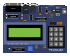
\includegraphics[scale=1.0]{img/logo.png} \\ PICSimLab \PNversion}
\author{Luis Claudio Gambôa Lopes  <lcgamboa@yahoo.com>\\
\\
{\centering Download: \href{https://github.com/lcgamboa/picsimlab}{github}}
\\
\ifpdf
\\
{\centering \href{https://lcgamboa.github.io/picsimlab\_docs/\PNversion/}{HTML version of documentation}} 
\else
\\
{\centering \hrefb{picsimlab.pdf}{PDF version of documentation}} 
\fi
\\
\\
{\centering \href{https://twitter.com/PICSimLab}{PICSimLab on Twitter}}
\\
\\
{\centering \href{https://discord.gg/fMT8szFYq7}{PICSimLab on Discord}}
}

\date{\today}


 \hypersetup{
     colorlinks,
     linkcolor={red!50!black},
     citecolor={blue!50!black},
     urlcolor={blue!80!black}
}


\definecolor{fore}{HTML}{1f497d}
\definecolor{codec}{HTML}{ffffcc}
\definecolor{colorbash}{rgb}{0.94,0.94,0.94}


%\includeonly{how_to_board}

\begin{document}

%begin{latexonly}
\def\hrefb#1#2{\href{#1}{#2}}
\def\hrefr#1#2{\href{run:#1}{#2}}
%end{latexonly}


\maketitle

\ifdefined\HCode\else
\tableofcontents
\fi

\chapter{Introduction}


PICSimLab means Programmable IC Simulator Laboratory

PICSimLab is a realtime emulator of \hyperlink{def:boards}{development boards} with integrated 
MPLABX/avr-gdb debugger. 
PICSimLab supports microcontrollers of \href{https://github.com/lcgamboa/picsim}{picsim} , 
\href{https://github.com/buserror/simavr}{simavr}, \href{http://mazsola.iit.uni-miskolc.hu/\%7edrdani/embedded/ucsim/}{uCsim}, 
\href{http://gpsim.sourceforge.net/}{gpsim}, \href{http://beckus.github.io/qemu_stm32/}{qemu-stm32} and 
\href{https://github.com/a159x36/qemu}{qemu-esp32} simulators.
PICSimLab have integration with MPLABX/Arduino IDE for programming the boards microcontrollers.
As the purpose of PICSimLab is to emulate real hardware it does not have any source code editing support.
For code editing and debugging the same tools used for a real board should be used with PICSimLab, such as
MPLABX, Arduino IDE or VSCode with PlatformIO. 

PICSimLab supports several devices (spare parts) that can be connected to the boards for simulation. 
As for example LEDs and push buttons for simple outputs and inputs and some more complex ones like the ethernet 
shield w5500 for internet connection or the color graphic display ili9340 with touchscreen. 
The the complete list of parts can be accessed in the chapter \hyperlink{def:spare}{Spare Parts}. 



\begin{figure}[H]
\center
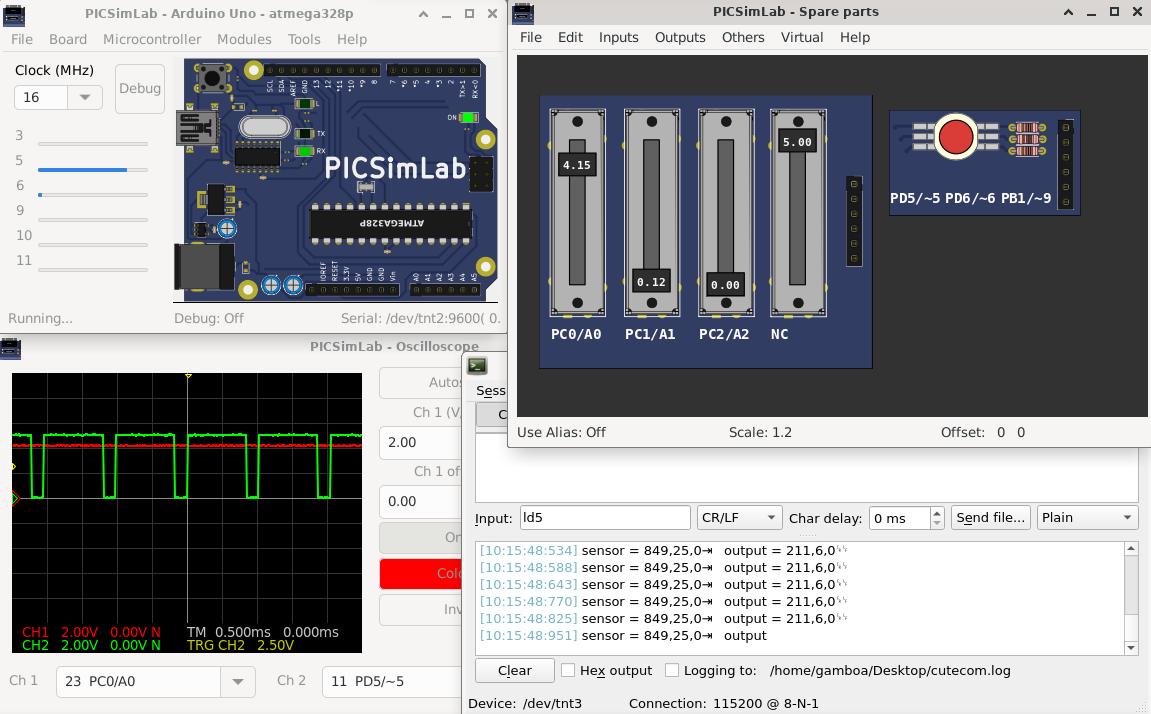
\includegraphics[width=0.99\textwidth]{img/screenshot.png} 
\end{figure} 

\chapter{Install}

\section{Stable version executables download} 

If you are on Linux or Windows you can download the last version at:

\href{https://github.com/lcgamboa/picsimlab/releases}{https://github.com/lcgamboa/picsimlab/releases}

If you are on macOS you can run PICSimLab using Wine:

\begin{enumerate}
 \item  Download and install [`xquartz`](https://www.xquartz.org)
 \item  Download and install [Wine](https://dl.winehq.org/wine-builds/macosx/download.html)
 \item  Download the executable and double-click it to run the installer
\end{enumerate}

\section{Unstable version executables download}

The binaries of last code available on github can be downloaded at: \href{https://sourceforge.net/projects/picsim/files/latest\%20code\%20build\%20\%28unstable\%29/}{Sourceforge.net}
 
The unstable test version have the unreleased features of \href{https://github.com/lcgamboa/picsimlab/blob/master/CHANGELOG_auto.md}{Changelog\_auto.md}

If you need a specific binary that is not available please contact me. 

\section{Install from source}\hypertarget{def:isource}{}

\subsection{Linux}

 In Debian Linux and derivatives Linux native:

\textbf{Using a user with permission to run the sudo command:}

In first time build:
\begin{minted}[baselinestretch=1.2,fontsize=\footnotesize,bgcolor=colorbash]{bash}
git clone --depth=1 https://github.com/lcgamboa/picsimlab.git
cd picsimlab
bscripts/build_all_and_install.sh
\end{minted}

To recompile use:
\begin{minted}[baselinestretch=1.2,fontsize=\footnotesize,bgcolor=colorbash]{bash}
make -j4
\end{minted}

\subsection{Windows}

 Cross-compiling for Windows (from Linux or \href{https://docs.microsoft.com/windows/wsl/install-win10}{WSL} on win10)

In first time build in Debian Linux and derivatives target Windows 64 bits:

 \begin{minted}[baselinestretch=1.2,fontsize=\footnotesize,bgcolor=colorbash]{bash}
git clone https://github.com/lcgamboa/picsimlab.git
cd picsimlab
bscripts/build_w64.sh
\end{minted}

To recompile use:

\begin{minted}[baselinestretch=1.2,fontsize=\footnotesize,bgcolor=colorbash]{bash}
make FILE=Makefile.cross -j4 
\end{minted}

For target Windows 32 bits:

\begin{minted}[baselinestretch=1.2,fontsize=\footnotesize,bgcolor=colorbash]{bash}
git clone https://github.com/lcgamboa/picsimlab.git
cd picsimlab
bscripts/build_w32.sh
\end{minted}

To recompile use:
\begin{minted}[baselinestretch=1.2,fontsize=\footnotesize,bgcolor=colorbash]{bash}
make FILE=Makefile.cross_32 -j4 
\end{minted}

\subsection{macOS}

Theoretically it is possible to compile PICSimLab natively on macOS. But I do not have access to any computer
 with macOS to try to compile and until today nobody has communicated that they managed to do it. (help wanted) 


\subsection{Experimental version}

Experimental version can be built using the parameter "exp" on scripts:
\begin{minted}[baselinestretch=1.2,fontsize=\footnotesize,bgcolor=colorbash]{bash}
bscripts/build_all_and_install.sh exp
bscripts/build_w64.sh exp
bscripts/build_w32.sh exp
\end{minted}
And recompiled using the parameter "exp" on Makefiles:
\begin{minted}[baselinestretch=1.2,fontsize=\footnotesize,bgcolor=colorbash]{bash}
make -j4 exp
make FILE=Makefile.cross -j4  exp
make FILE=Makefile.cross_32 -j4 exp
\end{minted}
 


\chapter{Simulator Interface}

\section{Main Window}

The main window consists of a menu, a status bar, a frequency selection combobox, an on/off button to trigger debugging, some board-specific controls and the part of the board interface itself.

In the title of the window is shown the name of the simulator PICSimLab, followed by the board and the microcontroller in use.


\begin{figure}[H]
\center
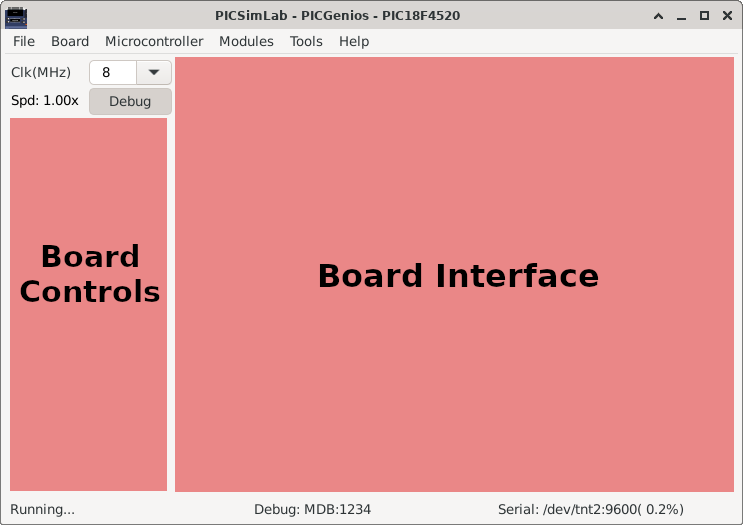
\includegraphics[width=0.99\textwidth]{img/int.png} 
\end{figure} 

The frequency selection combobox directly changes the working speed of the microcontroller.
The ``Spd'' label show the ratio between simulation speed and real time. when the ``Spd'' label goes red indicates that the computer is not being able to run the program in real time for the selected clock. 
In this case the simulation may present some difference than expected and the CPU load will be increased.

The on/off button to enable debugging is used to enable debugging support, when active simulation load is increased.

The menus and their functions are listed below:
\begin{itemize}
\item File
\begin{itemize}
\item Load Hex - Load .hex files
\item Reload Last - Reload the last used .hex file
\item Save Hex - Save memory in a .hex file
\item Configure - Open the configuration windows
\item Save Workspace - Saves all current workspace settings to a .pzw file
\item Load Workspace - Loads saved settings from a .pzw file
\item Exit
\end{itemize}
\item Board
\begin{itemize}
\item Arduino Uno - Choose board Arduino Uno
\item Breadboard - Choose board Breadboard
\item Franzininho - Choose board Franzininho
\item K16F - Choose board K16F
\item McLab1 - Choose board McLab1
\item McLab2 - Choose board McLab2
\item PICGenios - Choose board PICGenios
\item PQDB - Choose board PQDB
\end{itemize}
\item Microcontroller
\begin{itemize}
 \item xxxxx - Selects the microcontroller to be used (depends on the selected board)
\end{itemize}
\item Modules
\begin{itemize}
\item Oscilloscope - Open the oscilloscope window
\item Spare parts - Open the spare parts window
\end{itemize}
\item Tools 
\begin{itemize}
 \item Serial Terminal - Open the serial terminal \hyperlink{def:sterm}{Cutecom}
 \item Serial Remote Tank - Open the \hyperlink{def:srtank}{remote tank simulator}
 \item Esp8266 Modem Simulator -  Open the \hyperlink{def:espmsim}{Esp8266 Modem Simulator}
 \item Arduino Bootloader - Load microcontroller with \hyperlink{def:aboot}{Arduino serial bootloader} 
 \item MPLABX Debugger Plugin - Open the web page to download the \hyperlink{def:mpdebug}{MPLABX Debugger Plugin} 
 \item Pin Viewer - Open the \hyperlink{def:pinv}{Pin Viewer} 
\end{itemize}
\item Help 
\begin{itemize}
 \item Contents - Open the Help window
 \item Board - Open the Board Help window
 \item Examples - Load the examples
 \item About Board - Show message about author and version of board
 \item About PICSimLab - Show message about author and version of PICSimLab
\end{itemize}
\end{itemize}


\begin{figure}[H]
\center
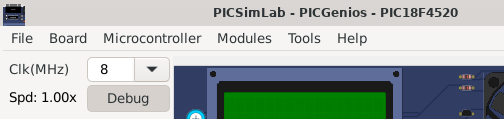
\includegraphics[width=0.85\textwidth]{img/int1.png} 
\end{figure} 

The first part of the status bar shows the state of the simulation, in the middle part the status of the debug support and in the last part the name of the serial port used, its default speed and the error in relation to the real speed configured in the microcontroller.

\begin{figure}[H]
\center
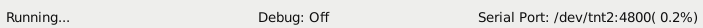
\includegraphics[width=0.85\textwidth]{img/int2.png} 
\end{figure} 


\section{Interaction with the Board}

On the interface area of the board it is possible to interact in some ways:

\begin{itemize}
 \item Click in ICSP connector to load an .hex file.
 \item Click in PWR button to ON/OFF the emulator..
 \item The buttons can be activated through mouse or keys 1, 2, 3 e 4.
 \item Click and drag in potentiometers to change their values.
 \item Click on EEPROM memory to view its contents.
\end{itemize}


\section{Command Line}

PICSimLab supports two command lines format:

One for load a PICSimLab Workspace file (.pzw) 
\begin{minted}[baselinestretch=1.2,fontsize=\footnotesize,bgcolor=colorbash]{bash}
  picsimlab file.pzw
\end{minted}

And other for load .hex files
\begin{minted}[baselinestretch=1.2,fontsize=\footnotesize,bgcolor=colorbash]{bash}
  picsimlab boardname microcontroller [file.hex] [file.pcf]
\end{minted}


\section{Remote Control Interface}\hypertarget{def:rcontrol}{}

The remote control interface allows other programs to control the PICSimLab simulation
through a TCP/IP socket using text formatted commands. 

The PICSimLab remote control interface supports TCP connections using telnet or nc (netcat).

The default port is 5000 and can be changed in configuration windows. 

The 'rlwrap' command can be used for best command edition support in telnet or nc:
\begin{minted}[baselinestretch=1.2,fontsize=\footnotesize,bgcolor=colorbash]{bash}
 rlwrap nc 127.0.0.1 5000
\end{minted}
  
The supported commands can be shown using the ``help'' command:  
\begin{minted}[baselinestretch=1.2,fontsize=\footnotesize,bgcolor=colorbash]{bash}
 help
List of supported commands:
  dumpe [a] [s]- dump internal EEPROM memory
  dumpf [a] [s]- dump Flash memory
  dumpr [a] [s]- dump RAM memory
  exit         - shutdown PICSimLab
  get ob       - get object value
  help         - show this message
  info         - show actual setup info and objects
  loadhex file - load hex file (use full path)  
  pins         - show pins directions and values
  pinsl        - show pins formated info
  quit         - exit remote control interface
  reset        - reset the board
  set ob vl    - set object with value
  sync         - wait to syncronize with timer event
  version      - show PICSimLab version
Ok
\end{minted}
  

The ``info'' command show all available "objects" and values:
\begin{minted}[baselinestretch=1.2,fontsize=\footnotesize,bgcolor=colorbash]{bash}
info
Board:     Arduino Uno
Processor: atmega328p
Frequency:   16000000 Hz
Use Spare: 1
    board.out[00] LD_L= 254
  part[00]: LEDs
    part[00].out[08] LD_1= 254
    part[00].out[09] LD_2= 30
    part[00].out[10] LD_3= 254
    part[00].out[11] LD_4= 254
    part[00].out[12] LD_5 254
    part[00].out[13] LD_6= 254
    part[00].out[14] LD_7= 254
  part[01]: Buzzer
    part[01].out[02] LD_1= 140
  part[02]: Push buttons
    part[02].in[00] PB_1= 1
    part[02].in[01] PB_2= 0
    part[02].in[02] PB_3= 1
    part[02].in[03] PB_4= 1
    part[02].in[04] PB_5= 1
    part[02].in[05] PB_6= 1
    part[02].in[06] PB_7= 1
    part[02].in[07] PB_8= 1
Ok
\end{minted}

The ``pins'' command show all pins directions and digital values:
\begin{minted}[baselinestretch=1.2,fontsize=\footnotesize,bgcolor=colorbash]{bash}
pins
  pin[01] ( PC6/RST) < 0                 pin[15] (  PB1/~9) > 0 
  pin[02] (   PD0/0) < 1                 pin[16] ( PB2/~10) > 0 
  pin[03] (   PD1/1) < 1                 pin[17] ( PB3/~11) > 0 
  pin[04] (   PD2/2) < 1                 pin[18] (  PB4/12) < 0 
  pin[05] (  PD3/~3) > 0                 pin[19] (  PB5/13) > 0 
  pin[06] (   PD4/4) < 1                 pin[20] (     +5V) < 1 
  pin[07] (     +5V) < 1                 pin[21] (    AREF) < 0 
  pin[08] (     GND) < 0                 pin[22] (     GND) < 0 
  pin[09] (  PB6/X1) < 0                 pin[23] (  PC0/A0) < 0 
  pin[10] (  PB7/X2) < 0                 pin[24] (  PC1/A1) < 0 
  pin[11] (  PD5/~5) < 1                 pin[25] (  PC2/A2) < 0 
  pin[12] (  PD6/~6) < 1                 pin[26] (  PC3/A3) < 0 
  pin[13] (   PD7/7) < 1                 pin[27] (  PC4/A4) > 0 
  pin[14] (   PB0/8) > 0                 pin[28] (  PC5/A5) > 0 
Ok
\end{minted}

The ``pinsl'' command show all pins info in text formatted output:
\begin{minted}[baselinestretch=1.2,fontsize=\footnotesize,bgcolor=colorbash]{bash}
pinsl
28 pins [atmega328p]:
  pin[01] D I 0 000 0.000 "PC6/RST " 
  pin[02] D I 1 200 0.000 "PD0/0   " 
  pin[03] D I 1 200 0.000 "PD1/1   " 
  pin[04] D I 1 200 0.000 "PD2/2   " 
  pin[05] D O 0 007 0.000 "PD3/~3  " 
  pin[06] D I 1 200 0.000 "PD4/4   " 
  pin[07] P I 1 200 0.000 "+5V     " 
  pin[08] P I 0 000 0.000 "GND     " 
  pin[09] D I 0 000 0.000 "PB6/X1  " 
  pin[10] D I 0 000 0.000 "PB7/X2  " 
  pin[11] D I 1 200 0.000 "PD5/~5  " 
  pin[12] D I 1 200 0.000 "PD6/~6  " 
  pin[13] D I 1 200 0.000 "PD7/7   " 
  pin[14] D O 0 000 0.000 "PB0/8   " 
  pin[15] D O 0 000 0.000 "PB1/~9  " 
  pin[16] D O 0 000 0.000 "PB2/~10 " 
  pin[17] D O 0 006 0.000 "PB3/~11 " 
  pin[18] D I 0 000 0.000 "PB4/12  " 
  pin[19] D O 0 000 0.000 "PB5/13  " 
  pin[20] P I 1 200 0.000 "+5V     " 
  pin[21] R I 0 000 0.000 "AREF    " 
  pin[22] P I 0 000 0.000 "GND     " 
  pin[23] A I 0 000 0.875 "PC0/A0  " 
  pin[24] A I 0 000 1.925 "PC1/A1  " 
  pin[25] A I 0 000 2.700 "PC2/A2  " 
  pin[26] A I 0 000 4.275 "PC3/A3  " 
  pin[27] D O 1 179 0.000 "PC4/A4  " 
  pin[28] D O 1 186 0.000 "PC5/A5  " 
Ok
\end{minted}


You can view one input/output state using the ``get'' command:
\begin{minted}[baselinestretch=1.2,fontsize=\footnotesize,bgcolor=colorbash]{bash}
get board.out[00]

get part[02].in[01]
\end{minted}

Its possible use the ``get'' command to view individual pins state:
\begin{minted}[baselinestretch=1.2,fontsize=\footnotesize,bgcolor=colorbash]{bash}
#digital state
get pin[19]
pin[19]= 0 
Ok

#digital mean value (0-200)
get pinm[19]
pin[18]= 100 
Ok

#analog state
get apin[25]
apin[25]= 2.700
Ok

#all info
get pinl[13]
pin[13] D I 1 200 0.000 "PD7/7   "
Ok
\end{minted}



And set value of one input using the ``set'' command:
\begin{minted}[baselinestretch=1.2,fontsize=\footnotesize,bgcolor=colorbash]{bash}
set part[02].in[01]  0
set part[02].in[01]  1
\end{minted}

Or set value of one pin using the ``set'' command:
\begin{minted}[baselinestretch=1.2,fontsize=\footnotesize,bgcolor=colorbash]{bash}
#digital
set pin[10]  2

#analog
set apin[20] 2.345
\end{minted}



For windows users \href{https://www.putty.org/}{putty telnet client} is a good option 
to access the remote control interface. 


\section{Picture Map Reference}\hypertarget{def:map}{}

Names used in .map files for boards and parts are standardized and used by the remote control interface. 

The names must start with \textbf{I\_} if it is an input, \textbf{O\_} if it is an output or \textbf{B\_} if it
is bidirectional. 
And be followed by one of the two-letter types in the table below before the area name. 

{%
\newcommand{\mc}[3]{\multicolumn{#1}{#2}{#3}}
\begin{center}
\begin{tabular}{cclcc}
\textbf{Function} & \textbf{Type} & \mc{1}{c}{\textbf{Description}} & \textbf{RControl In} & \textbf{RControl Out}\\
I & MD & Memory Dump & - & -\\
I & KB & Keyboard Key & 0 or 1 & 0 or 1\\
I & PG & Program & - & -\\
I & CN & Connector & - & -\\
B & PO & Potentiometer & 0 to 200 & 0 to 200\\
B & JP & Jumper & 0 or 1 & 0 or 1\\
B & VS & Value short & -32768 to 32767 & -32768 to 32767\\
B & PB & Push button & 0 or 1 & 0 or 1\\
B & DP & Dip switch & 0 or 1 & 0 or 1\\
B & SW & Switch & 0 or 1 & 0 or 1\\
B & RT & Rotary encoder & 0 to 200 & 0 to 200\\
B & AJ & Dip switch & - & -\\
O & MC & Motor Cooler & - & 0 to 200\\
O & PN & Pin name & - & -\\
O & ST & Status & - & -\\
O & IC & IC name & - & -\\
O & LR & LED RGB & - & -\\
O & LM & LED Matrix & - & -\\
O & DI & Display Info & - & -\\
O & LD & LED & - & 0 to 200\\
O & DS & Display & - & if alphanumeric show text\\
O & MT & DC motor & - & dir 0 or 1, spd. 0 to 200, pos. 0 to 200\\
O & DG & Degree & - & float angle\\
O & SS & seven segment & - & decoded number\\
\end{tabular}
\end{center}
}
 

For example area named \textbf{B\_PB\_Start}, which describes the position of a push button named "Start". 
The \textbf{B\_} bidirectional indicates that the mapped area serves as user action input and drawing output.  
 

\chapter{Boards} \hypertarget{def:boards}{}

PICSimLab currently supports five backend simulators. The stable version supports 
\href{https://github.com/lcgamboa/picsim}{picsim} and \href{https://github.com/buserror/simavr}{simavr}. 
The experimental version supports \href{http://mazsola.iit.uni-miskolc.hu/\%7edrdani/embedded/ucsim/}{uCsim}, 
\href{http://gpsim.sourceforge.net/}{gpsim} and \href{http://beckus.github.io/qemu_stm32/}{qemu-stm32} in 
addition to the stable ones.

The Figure below shows which cards are based on which backend simulator:

\begin{figure}[H] 
\center
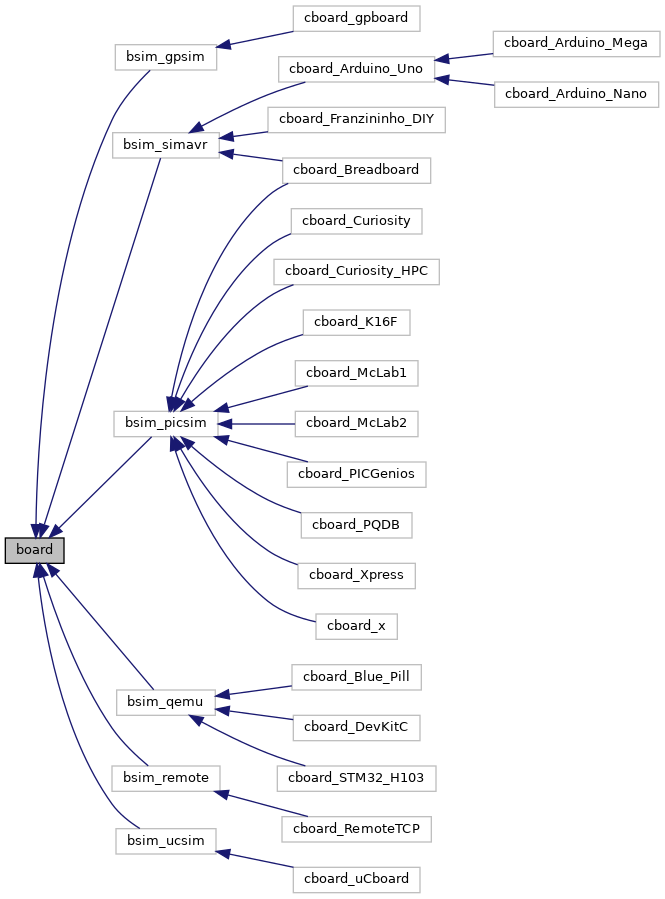
\includegraphics[width=0.65\textwidth]{img/boards.png} 
\caption{Boards backend simulators}
\end{figure} 

The below table show the supported debug interface of each simulator:

\begin{center}
\begin{tabular}{c|c}
\hline \textbf{Backend} & \textbf{Debug Support}\\
\hline picsim & see the section \hyperlink{def:mplabxd}{MPLABX Integrated Debug}\\
\hline simavr & see the sections \hyperlink{def:mplabxd}{MPLABX Integrated Debug} and \hyperlink{def:gdbavr}{remote avr-gdb Debug}\\
\hline qemu-stm32 & see the section \hyperlink{def:gdbarm}{remote arm-gdb Debug}\\
\hline uCsim & see the section \hyperlink{def:ucsim}{uCsim remote console (telnet) Debug}\\
\hline gpsim & none yet\\
\hline 
\end{tabular}
\end{center}



\section{Breadboard}

It is a generic board only with reset, serial and crystal circuits and support to multiple microcontrollers 
of \href{https://github.com/lcgamboa/picsim}{picsim} and \href{https://github.com/buserror/simavr}{simavr}.

\begin{figure}[H]
\center
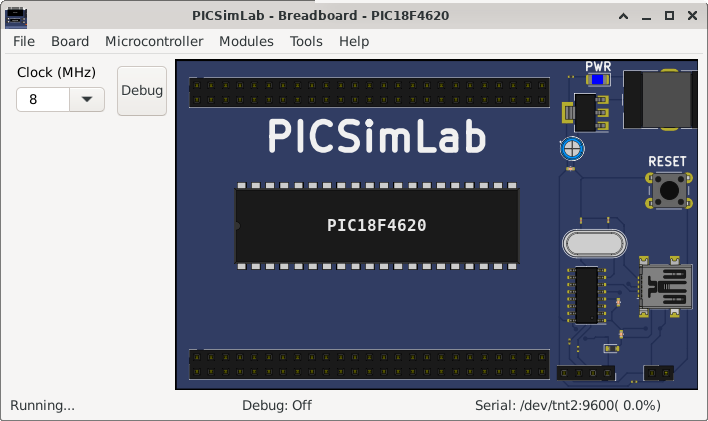
\includegraphics[width=0.7\textwidth]{img/picsimlab0.png} 
\end{figure} 

\hrefb{pdf/boards/Breadboard.pdf}{Board Breadboard schematics}.\vspace{0.5cm}

\href{https://lcgamboa.github.io/picsimlab_examples/board_Breadboard.html}{Examples}

\section{McLab1}

It emulates the Labtools development board McLab1 that uses one PIC16F84, PIC16F628 or PIC16F648 of \href{https://github.com/lcgamboa/picsim}{picsim}.

\begin{figure}[H]
\center
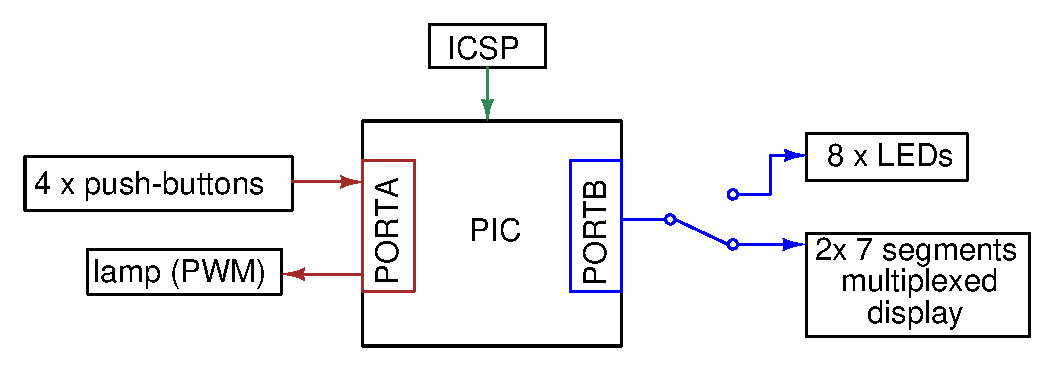
\includegraphics[width=0.85\textwidth]{img/blocks_p1.eps} 
\end{figure} 


\begin{figure}[H]
\center
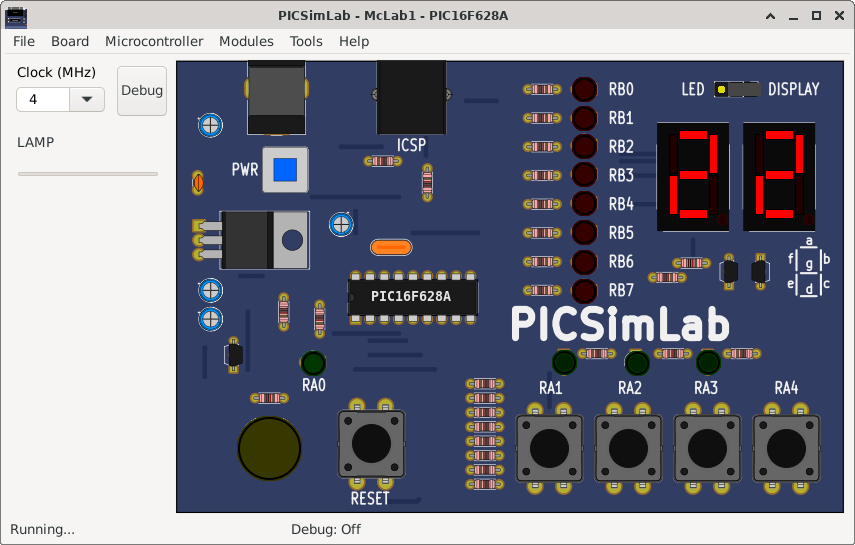
\includegraphics[width=0.7\textwidth]{img/picsimlab1.png} 
\end{figure} 

\hrefb{pdf/boards/McLab1.pdf}{Board McLab1 schematics}.\vspace{0.5cm}

The code examples can be loaded in PICSimLab menu \textbf{Help->Examples}.

The source code of board McLab1 examples using \href{http://www.microchip.com/mplabx}{MPLABX and XC8} compiler 
are in the link: \href{https://lcgamboa.github.io/picsimlab_examples/board_McLab1.html}{board\_McLab1}.

\section{K16F}

It emulates an didactic board developed by author that uses one PIC16F84, PIC16F628 or PIC16F648 of \href{https://github.com/lcgamboa/picsim}{picsim}.

\begin{figure}[H]
\center
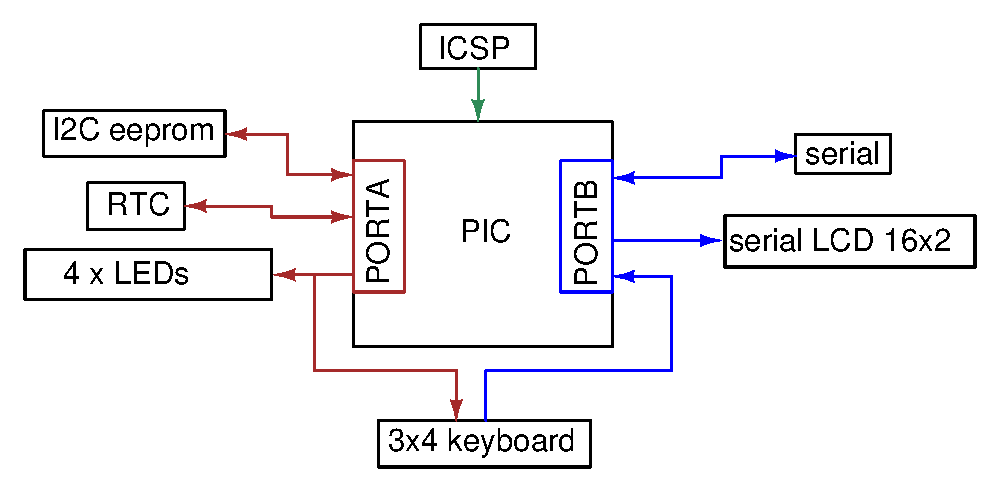
\includegraphics[width=0.85\textwidth]{img/blocks_p2.eps} 
\end{figure} 


\begin{figure}[H]
\center
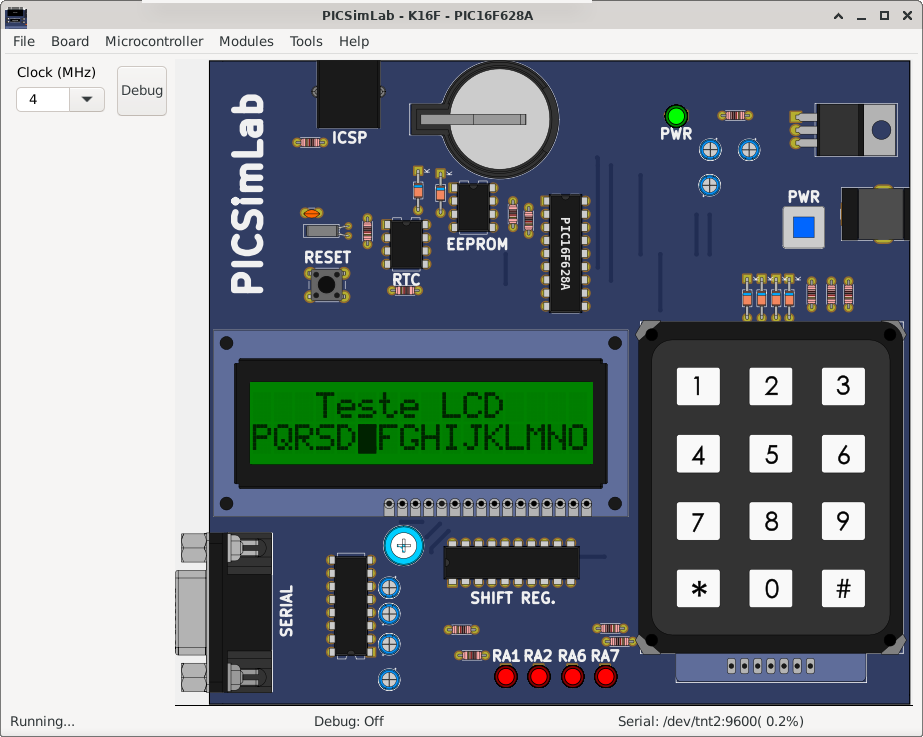
\includegraphics[width=0.8\textwidth]{img/picsimlab2.png} 
\end{figure} 

\hrefb{pdf/boards/K16F.pdf}{Board K16F schematics}.\vspace{0.5cm}

The code examples can be loaded in PICSimLab menu \textbf{Help->Examples}.

The source code of board K16F examples using \href{http://www.microchip.com/mplabx}{MPLABX and XC8} compiler are in
the link: \href{https://lcgamboa.github.io/picsimlab_examples/board_K16F.html}{board\_K16F}.


\section{McLab2}

It emulates the Labtools development board McLab2 that uses one PIC16F777, PIC16F877A, PIC18F452, PIC18F4520, PIC18F4550 or PIC18F4620 of \href{https://github.com/lcgamboa/picsim}{picsim}.

\begin{figure}[H]
\center
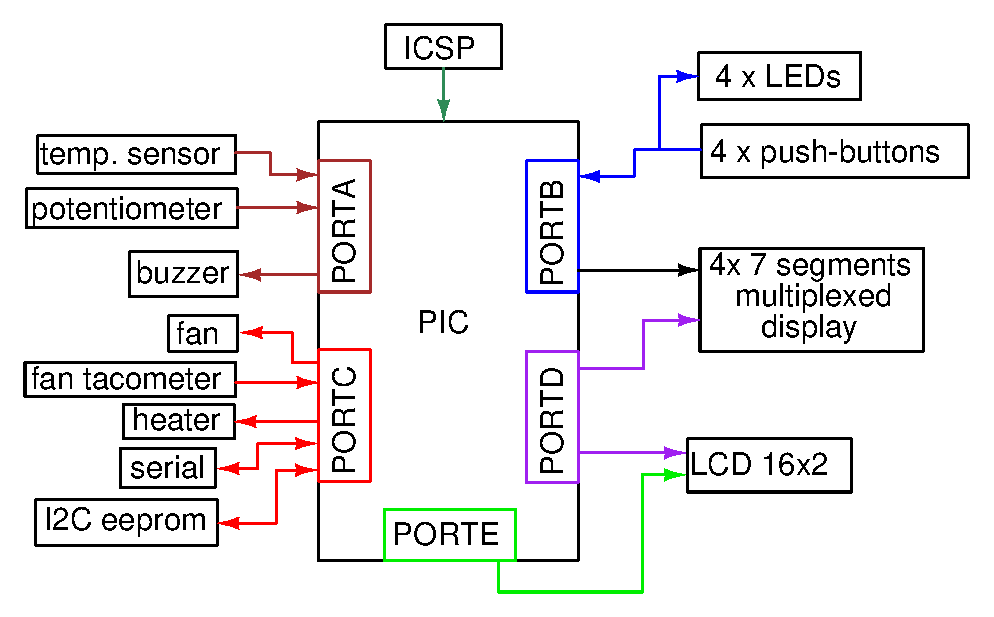
\includegraphics[width=0.85\textwidth]{img/blocks_p3.eps} 
\end{figure} 


\begin{figure}[H]
\center
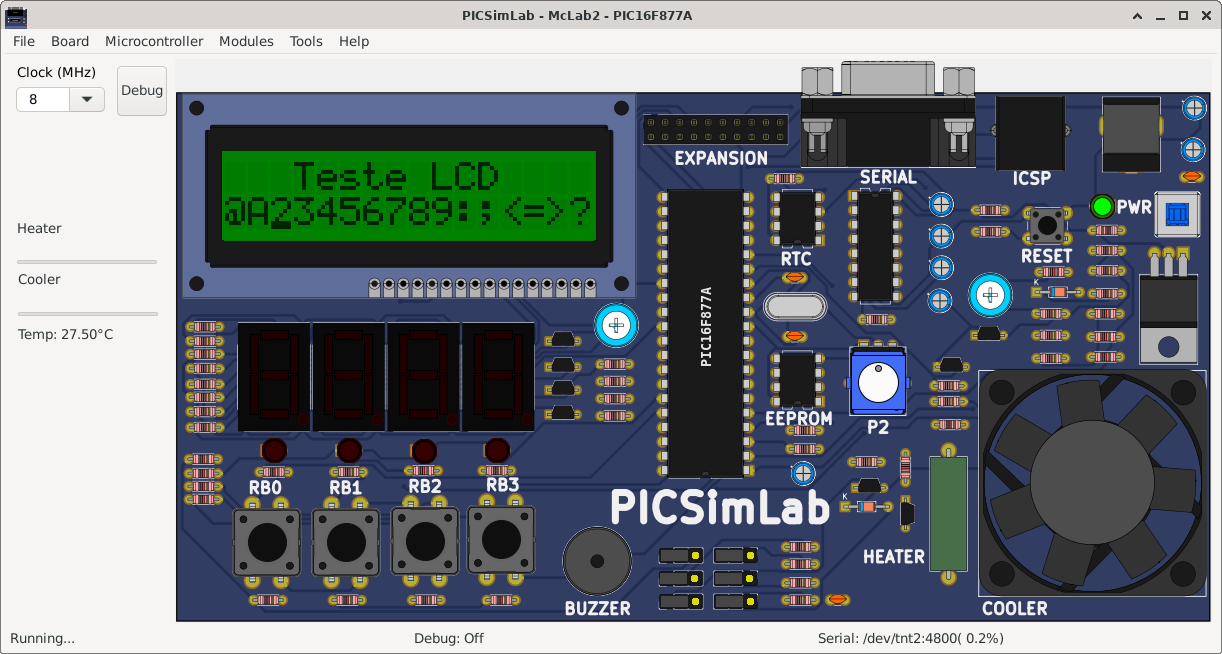
\includegraphics[width=0.9\textwidth]{img/picsimlab3.png} 
\end{figure} 

\hrefb{pdf/boards/McLab2.pdf}{Board McLab2 schematics}.\vspace{0.5cm}

The code examples can be loaded in PICSimLab menu \textbf{Help->Examples}.

The source code of board McLab2 examples using \href{http://www.microchip.com/mplabx}{MPLABX and XC8} 
compiler are in the link: \href{https://lcgamboa.github.io/picsimlab_examples/board_McLab2.html}{board\_McLab2}.

\section{PICGenios}

It emulates the microgenius development board PICGenios PIC18F e PIC16F Microchip that uses one PIC16F777, PIC16F877A, PIC18F452, PIC18F4520, PIC18F4550 or PIC18F4620 of \href{https://github.com/lcgamboa/picsim}{picsim}.

\begin{figure}[H]
\center
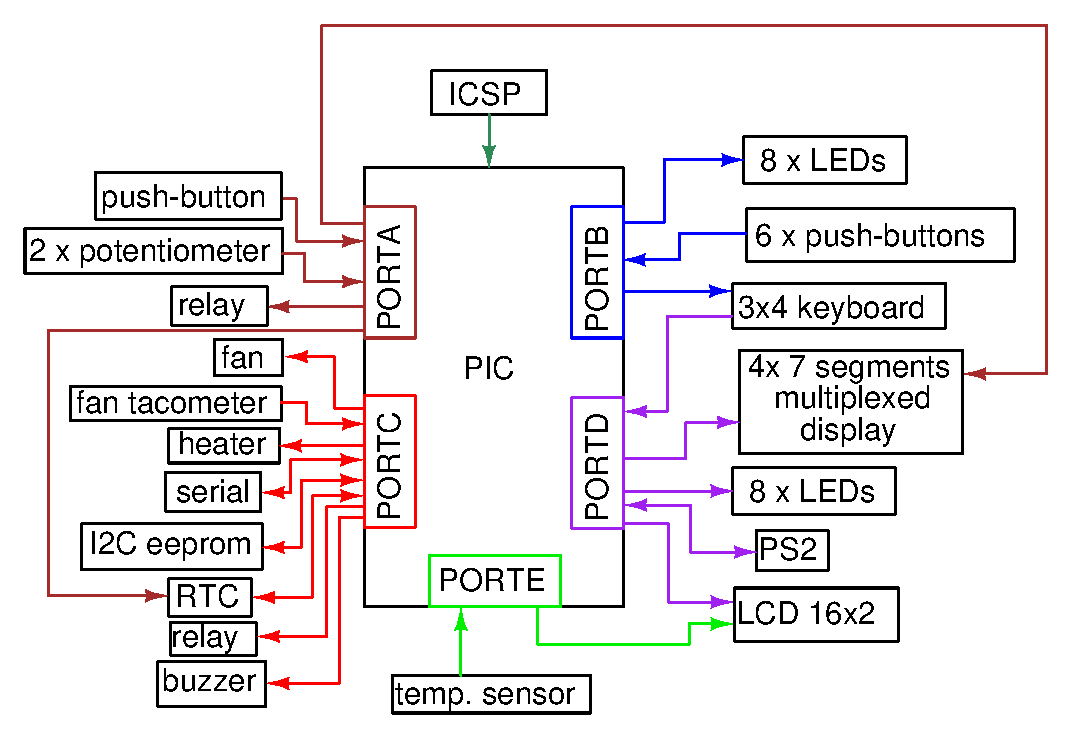
\includegraphics[width=0.85\textwidth]{img/blocks_p4.eps} 
\end{figure} 


\begin{figure}[H]
\center
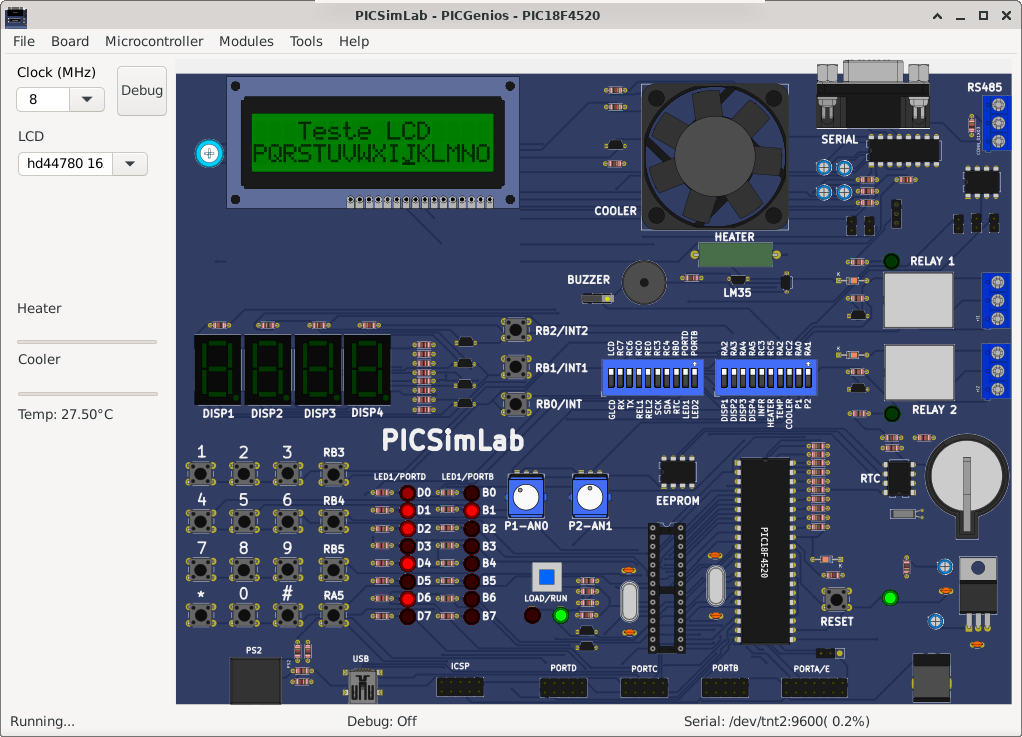
\includegraphics[width=0.99\textwidth]{img/picsimlab4.png} 
\end{figure} 

\hrefb{pdf/boards/PICGenios.pdf}{Board PICGenios schematics}.\vspace{0.5cm}

The code examples can be loaded in PICSimLab menu \textbf{Help->Examples}.

The source code of board PICGenios examples using 
\href{http://www.microchip.com/mplabx}{MPLABX and XC8} compiler are in the link: 
\href{https://lcgamboa.github.io/picsimlab_examples/board_PICGenios.html}{board\_PICGenios}.


\section{PQDB}

The PQDB board is an opensource/openhardware project, more info at \href{https://github.com/projetopqdb/}{https://github.com/projetopqdb/}.
It was developed to be used with arduino/freedom boards, but adapted to use the microcontroller PIC18F4520 of 
\href{https://github.com/lcgamboa/picsim}{picsim} on PICSImLab.

\begin{figure}[H]
\center
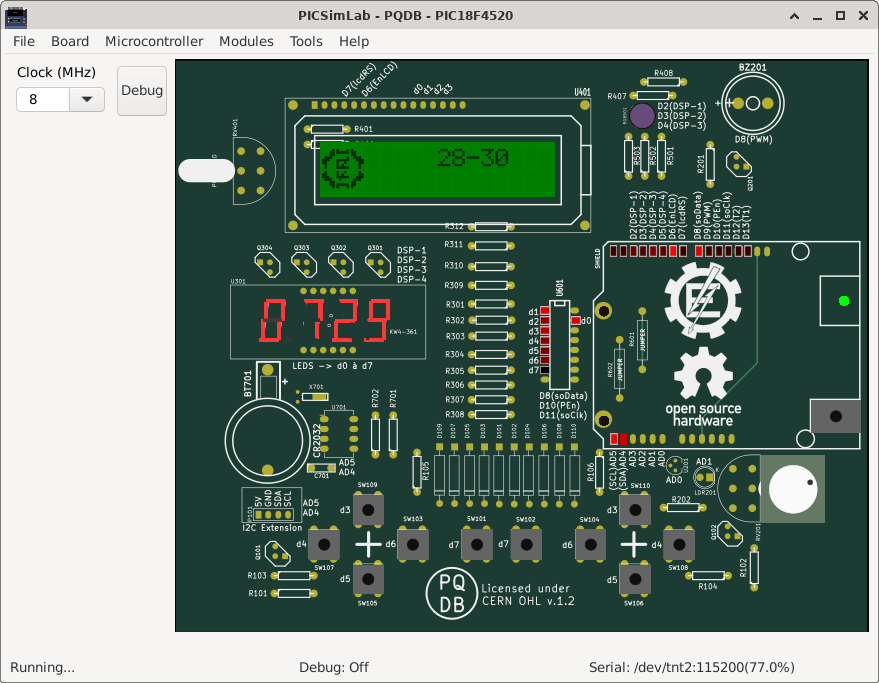
\includegraphics[width=0.99\textwidth]{img/board_PQDB.png} 
\end{figure} 

\hrefb{pdf/boards/PQDB.pdf}{Board PQDB schematics}.\vspace{0.5cm}

\hrefb{pdf/boards/PQDB_PIC18F.pdf}{Hat board PIC18F schematics}.\vspace{0.5cm}


\href{https://lcgamboa.github.io/picsimlab_examples/board_PQDB.html}{Examples}


\section{Arduino Uno}

It emulates the Arduino Uno development board that uses one ATMEGA328P microcontroller of \href{https://github.com/buserror/simavr}{simavr}.

\begin{figure}[H]
\center
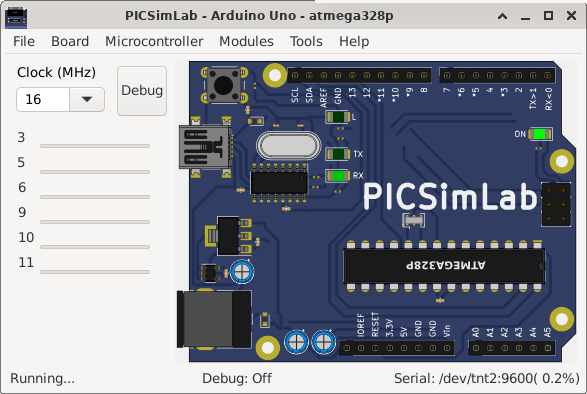
\includegraphics[width=0.80\textwidth]{img/picsimlab5.png} 
\end{figure} 

\href{https://www.arduino.cc/en/uploads/Main/Arduino_Uno_Rev3-schematic.pdf}{Board Arduino Uno schematics}.\vspace{0.5cm}

The code examples can be loaded in PICSimLab menu \textbf{Help->Examples}.

The source code of board Arduino Uno examples using the 
\href{https://www.arduino.cc/en/Main/Software}{Arduino IDE with avr-gcc} are in the link: 
\href{https://lcgamboa.github.io/picsimlab_examples/board_Arduino_Uno.html}{board\_Arduino\_Uno}.

More information about the Arduino in \href{https://www.arduino.cc/}{www.arduino.cc}

Information on how to configure the PICSimLab integration with the Arduino IDE can be found in the 
section: \hyperlink{def:arduinoide}{Arduino IDE Integration}.

\section{Franzininho DIY}

The Franzininho DIY board is an openhardware project, more info at \href{https://franzininho.com.br/}{https://franzininho.com.br/}.
It was developed to be used with the microcontroller ATtiny85 of 
of \href{https://github.com/buserror/simavr}{simavr}.

\begin{figure}[H]
\center
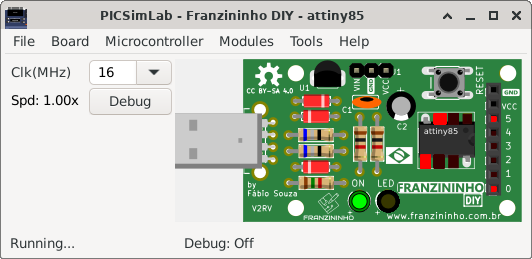
\includegraphics[width=0.7\textwidth]{img/board_Franzininho_DIY.png} 
\end{figure} 

\hrefb{pdf/boards/FranzininhoDIY.pdf}{Board Franzininho DIY schematics}.\vspace{0.5cm}

\href{https://lcgamboa.github.io/picsimlab_examples/board_Franzininho_DIY.html}{Examples}


\section{uCboard}

It is a generic board only with reset, serial and crystal circuits and support to multiple microcontrollers 
(initially C51, Z80 and STM8S103 )of \href{http://mazsola.iit.uni-miskolc.hu/\%7edrdani/embedded/ucsim/}{uCsim}.

\begin{figure}[H]
\center
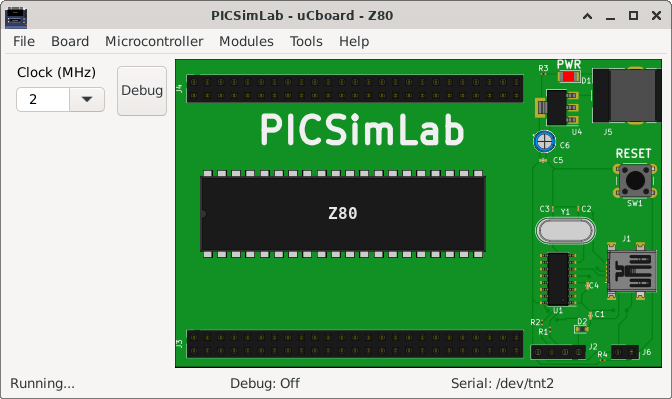
\includegraphics[width=0.7\textwidth]{img/uCboard.png} 
\end{figure} 

\href{https://lcgamboa.github.io/picsimlab_examples/board_uCboard.html}{Examples}


\section{Blue Pill}

It is a generic board only with reset, serial and crystal circuits and support to stm32f103c8t6 microcontroller of 
\href{https://beckus.github.io/qemu_stm32/}{qemu-stm32}.

\begin{figure}[H]
\center
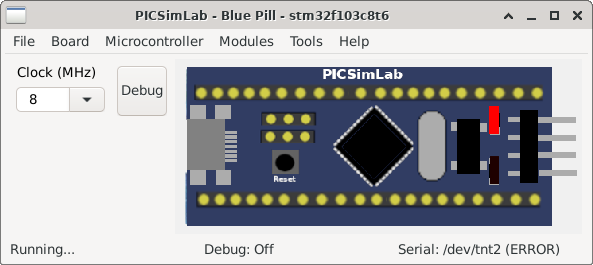
\includegraphics[width=0.7\textwidth]{img/Blue_Pill.png} 
\end{figure} 

\hrefb{pdf/boards/Blue_Pill.pdf}{Board Blue Pill schematics}.\vspace{0.5cm}

\href{https://lcgamboa.github.io/picsimlab_examples/board_Blue_Pill.html}{Examples}


\section{ESP32-DevKitC}

It is a simple board only with reset, serial and crystal circuits and support 
for ESP32 microcontroller of \href{https://github.com/a159x36/qemu}{qemu-esp32}.

\begin{figure}[H]
\center
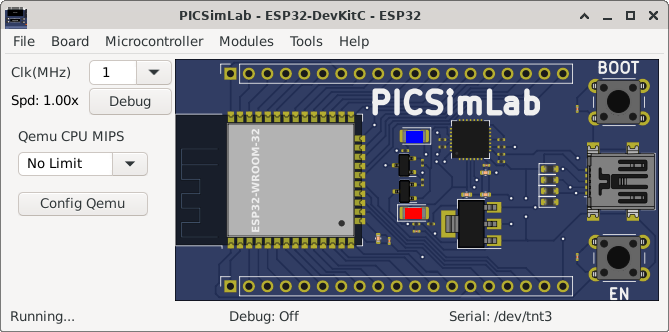
\includegraphics[width=0.7\textwidth]{img/DevKitC.png} 
\end{figure} 

\hrefb{pdf/boards/DevKitC.pdf}{Board DevKitC schematics}.\vspace{0.5cm}

For integrated use with the Arduino IDE or IDF esptool.py , simply configure the serial port as explained 
in the Chapter \hyperlink{def:seriali}{Serial Communication} to flash PICSimLab ESP32-DevKitC as a real ESP32 board.

\href{https://lcgamboa.github.io/picsimlab_examples/board_ESP32_DevKitC.html}{Examples}


\section{gpboard}

It is a generic board only with reset, serial and crystal circuits and support to multiple microcontrollers 
of \href{http://gpsim.sourceforge.net/}{gpsim}.

\begin{figure}[H]
\center
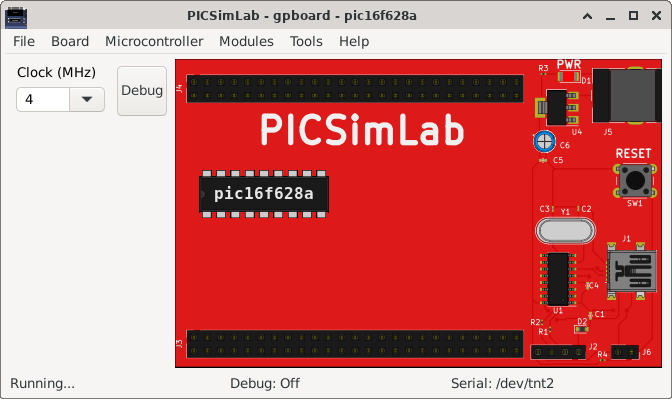
\includegraphics[width=0.7\textwidth]{img/gpboard.png} 
\end{figure} 

\href{https://lcgamboa.github.io/picsimlab_examples/board_gpboard.html}{Examples}


\section{STM32 H103}

It is a generic board only with reset, one push button, serial and crystal circuits and support to stm32f103rbt6 microcontroller of 
\href{https://beckus.github.io/qemu_stm32/}{qemu-stm32}.

\begin{figure}[H]
\center
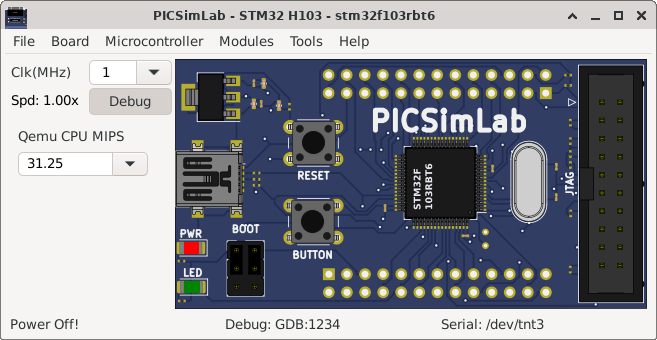
\includegraphics[width=0.7\textwidth]{img/STM32_H103.png} 
\end{figure} 

\hrefb{pdf/boards/STM32_H103.pdf}{Board STM32 H103 schematics}.\vspace{0.5cm}

\href{https://lcgamboa.github.io/picsimlab_examples/board_STM32_H103.html}{Examples}


\section{X}

It is a generic board, used as example in the tutorial 
\href{https://lcgamboa.github.io/picsimlab_docs/stable/CreatingNewBoards.html}{Creating New Boards}.

\begin{figure}[H]
\center
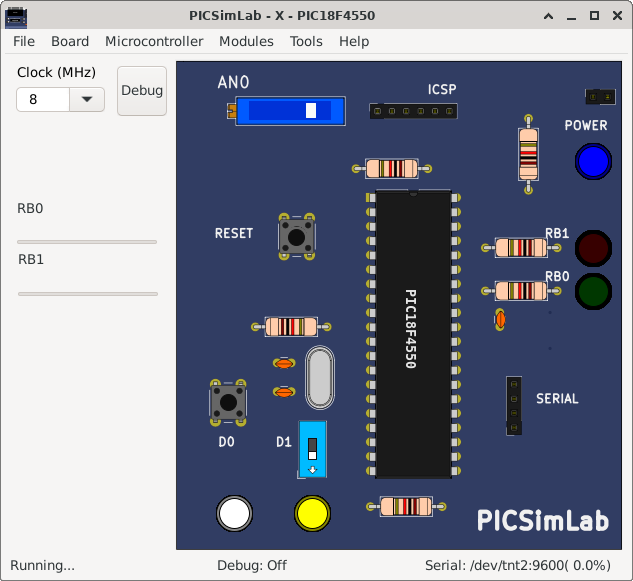
\includegraphics[width=0.7\textwidth]{img/X.png} 
\end{figure} 

\hrefb{pdf/boards/X.pdf}{Board X schematics}.\vspace{0.5cm}

\href{https://lcgamboa.github.io/picsimlab_examples/board_X.html}{Examples}

\chapter{Experimental Boards} \hypertarget{def:eboards}{}

Boards in the experimental phase. Probably with some bugs and missing features. 









\chapter{Serial Communication \label{seriali}} \hypertarget{def:seriali}{}

To use the simulator serial port emulation, you must install a NULL-MODEM emulator:

\begin{itemize}
 \item Windows: com0com \url{http://sourceforge.net/projects/com0com/}
 \item Linux: tty0tty  \url{https://github.com/lcgamboa/tty0tty}
 \end{itemize}

For communication the PICSimLab should be connected in one port of the NULL-MODEM emulator and the other application connected in the other port.
Configuration examples linking PICSimLab to \href{https://github.com/neundorf/CuteCom}{Cutecom} for serial communication:
 \vspace{0.5cm}
 
 \begin{tabular}{|c|c|c|c|c|}
 \hline OS&  PicsimLab port&  Cutecom port & NULL-Modem prog. &Connection\\
 \hline 
 \hline Windows&  com1 & com2 &com0com &com1<=>com2\\
 \hline Linux &  /dev/tnt2 & /dev/tnt3 &tty0tty &/dev/tnt2<=>/dev/tnt3\\
 \hline 
 \end{tabular}
 \vspace{0.5cm}
 
 The PICSimLab serial communication uses the 8N1 format.
 
 \section{Com0com Installation and Configuration(Windows)}
 
 Download the signed version of \href{https://sourceforge.net/projects/com0com/files/com0com/3.0.0.0/com0com-3.0.0.0-i386-and-x64-signed.zip/download}{com0com}.
 
Unzip the downloaded .zip file and run the specific installer of your operating system, x86 for windows 32-bit or x64 for windows 64-bit.
 
Configure the ``choose components'' window as the figure below:
 \begin{figure}[H]
\center
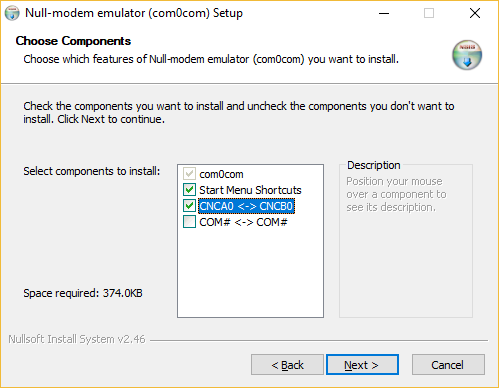
\includegraphics[width=0.8\textwidth]{img/com0com1.png} 
\end{figure} 


In the last configuration window, check the ``Launch setup'' option:
\begin{figure}[H]
\center
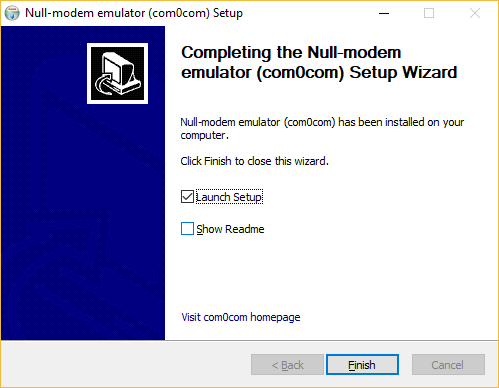
\includegraphics[width=0.8\textwidth]{img/com0com2.png} 
\end{figure} 

In the setup window, change the port names to COM1, COM2, COM3 ....
Just check the ``enable buffer overrun'' option on the two ports, click in the ``Apply'' button and close the setup.
In the configuration shown in the figure below, the COM1 and COM2 ports form a NULL-MODEM connection, where one port must be used by the PICSimLab and another by the application with serial communication.
\begin{figure}[H]
\center
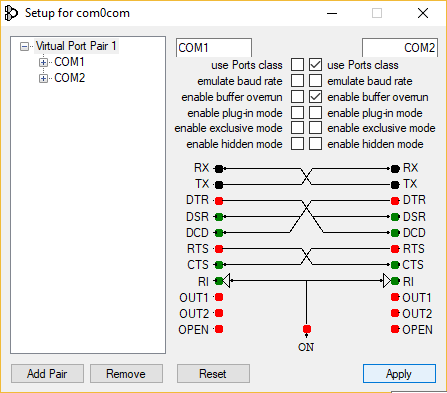
\includegraphics[width=0.8\textwidth]{img/com0com3.png} 
\end{figure} 
 
\section{tty0tty Installation and Configuration (Linux)}
 
Download the \href{https://github.com/lcgamboa/tty0tty/archive/master.zip}{tty0tyy}.
Unzip the downloaded folder.
 
Open a terminal and enter in the tty0tty/module/ folder and enter the following commands:
\begin{verbatim}
 sudo apt-get update
 sudo apt-get -y upgrade
 sudo apt-get -y install gcc make linux-headers-`uname -r` 
 sudo ./dkms-install.sh
 sudo modprobe tty0tty
\end{verbatim}

The user must be in the \textbf{dialout} group to access the ports. 
To add your user to \textbf{dialout} group use the command:
\begin{verbatim}
sudo usermod -a -G dialout your_user_name
\end{verbatim}
after this is necessary logout and login to group permissions take effect.


Once installed, the module creates 8 interconnected ports as follows:
\begin{verbatim}
  /dev/tnt0  <=>  /dev/tnt1 
  /dev/tnt2  <=>  /dev/tnt3 
  /dev/tnt4  <=>  /dev/tnt5 
  /dev/tnt6  <=>  /dev/tnt7 
\end{verbatim}

the connection between each pair is of the form:
\begin{verbatim}  
  TX   ->  RX
  RX   <-  TX 	
  RTS  ->  CTS
  CTS  <-  RTS
  DSR  <-  DTR
  CD   <-  DTR
  DTR  ->  DSR
  DTR  ->  CD
\end{verbatim}

Any pair of ports form a NULL-MODEM connection, where one port must be used by the PICSimLab and another by the application with serial communication.

\chapter{Backend Simulators}


PICSimLab currently supports five backend simulators:
\href{https://github.com/lcgamboa/picsim}{picsim},  
\href{https://github.com/buserror/simavr}{simavr}, 
\href{http://mazsola.iit.uni-miskolc.hu/\%7edrdani/embedded/ucsim/}{uCsim}, 
\href{http://gpsim.sourceforge.net/}{gpsim} and 
qemu (\href{https://beckus.github.io/qemu_stm32/}{stm32} and \href{https://github.com/a159x36/qemu}{esp32}).


The type of debug interface depends on the backend simulator utilized.

\section{PICsim} \hypertarget{def:PICSim}{}

``\href{https://github.com/lcgamboa/picsim}{PICsim} emulates some PIC microcontroller and periferics such as USART and timers, the simulator architecture permit easy implementation of external elements in c language. It can be used as a standalone simulator (picsim executable) or as a library in other programs (As in PICSimLab).''


\subsection{MPLABX Integrated Debug } \hypertarget{def:mplabxd}{}

To use the \href{http://www.microchip.com/mplabx}{MPLABX} IDE for debug and program the PicsimLab, install the plugin \href{https://github.com/lcgamboa/picsimlab_md/releases/}{com-picsim-picsimlab.nbm} in MPLABX.

The plugin connect to PICSimLab through a TCP socket using port 1234 (or other defined in configuration window), and you have to allow the access in the firewall.

\href{https://lcgamboa.github.io/picsimlab_docs/stable/UsewithMPLABX.html}{Tutorial: how to use MPLABX to program and debug PICsimLab}.


\section{simavr}\hypertarget{def:simavr}{}

``\href{https://github.com/buserror/simavr}{simavr} is a new AVR simulator for linux, or any platform that uses avr-gcc. It uses avr-gcc's own register definition to simplify creating new targets for supported AVR devices. The core was made to be small and compact, and hackable so allow quick prototyping of an AVR project. The AVR core is now stable for use with parts with <= 128KB flash, and with preliminary support for the bigger parts. The simulator loads ELF files directly, and there is even a way to specify simulation parameters directly in the emulated code using an .elf section. You can also load multipart HEX files.''

\subsection{avr-gdb Debug} \hypertarget{def:gdbavr}{}
 
 With debug support enabled you can use avr-gdb to debug the code used in the simulator. 
 Use the configuration window to choose between MDB (MPLABX) or GDB to debug AVR microcontrollers. 
 
 
 Use avr-gdb with the .elf file as the parameter:
 \begin{verbatim}
 avr-gdb compiled_file.elf
 \end{verbatim}
 and the command below to connect (1234 is the default port):
 \begin{verbatim}
 target remote localhost:1234
 \end{verbatim}

Graphic debug mode can be made using \href{https://www.eclipse.org/}{eclipse IDE} with \href{https://eclipse.baeyens.it/}{Sloeber Arduino plugin}.

It is also possible to debug using \href{https://platformio.org/}{platformIO in VSCode}, just add the configuration lines below in the project's \textbf{platformio.ini} file:
\begin{verbatim}
;upload_protocol = arduino
;upload_port = COM7
;upload_port = /dev/tnt3
;monitor_port = /dev/tnt3

upload_protocol = custom
upload_command = C:\"Program Files"\PicsimLab\picsimlab_tool.exe loadhex "$BUILD_DIR/firmware.hex"
;upload_command = /usr/bin/picsimlab_tool loadhex "$BUILD_DIR/firmware.hex"

build_type = debug
debug_tool = custom
debug_port = localhost:1234
debug_build_flags = -O2 -g
debug_init_break = tbreak setup
debug_init_cmds =
  define pio_reset_halt_target
  end
  define pio_reset_run_target
  end
  target extended-remote $DEBUG_PORT
  $LOAD_CMDS
  pio_reset_halt_target
  $INIT_BREAK
\end{verbatim}
%Compile, and upload the code to PICSimLab before starting Debug.

\subsection{MPLABX Int. Debug }
PICSimLab also supports using MPLABX to debug simavr. The configuration is the same as described in PICSim section: \hyperlink{def:mplabxd}{MPLABX Integrated Debug}. 
It's possible import and debug a Arduino sketch into MPLABX using the \href{https://github.com/janegilruud/chipKIT-importer-2.0}{Arduino import plugin}.

 \section{qemu-stm32} \hypertarget{def:qemu-stm32}{}
 ``\href{http://beckus.github.io/qemu_stm32/}{Qemu STM32}: QEMU with an STM32 microcontroller implementation''
 
 \subsection{arm-gdb Debug} \hypertarget{def:gdbarm}{}
 
 With debug support enabled you can use arm-none-eabi-gdb (or gdb-multiarch) to debug the code used in the simulator. 
 
 Use arm-none-eabi-gdb with the .elf file as the parameter:
 \begin{verbatim}
 arm-none-eabi-gdb compiled_file.elf
 \end{verbatim}
 and the command below to connect (1234 is the default port):
 \begin{verbatim}
 target extended-remote localhost:1234
 \end{verbatim}

Graphic debug mode can be made using \href{https://www.eclipse.org/}{eclipse IDE} with 
\href{https://projects.eclipse.org/projects/iot.embed-cdt}{Eclipse Embedded CDT} or using \href{https://platformio.org/}{platformIO in VSCode}, just add the configuration lines below in the project's \textbf{platformio.ini} file:
\begin{verbatim}
upload_protocol = custom
upload_command = C:\"Program Files"\PicsimLab\picsimlab_tool.exe loadbin "$BUILD_DIR/firmware.bin"
;upload_command = /usr/bin/picsimlab_tool loadbin "$BUILD_DIR/firmware.bin"

build_type = debug
debug_tool = custom
debug_port = localhost:1234
debug_build_flags = -O2 -g
debug_init_break = tbreak main
debug_init_cmds =
  define pio_reset_halt_target
      monitor system_reset
  end
  define pio_reset_run_target
      monitor system_reset
  end
  target extended-remote $DEBUG_PORT
  $LOAD_CMDS
  pio_reset_halt_target
  $INIT_BREAK
\end{verbatim}

\section{qemu-ESP32} \hypertarget{def:qemu-esp32}{}
 ``\href{https://github.com/a159x36/qemu}{Qemu ESP32}: Qemu Emulator for TTGO TDisplay esp32 board. ''
  
For integrated use with the Arduino IDE or IDF esptool.py , simply configure the serial port as explained 
in the Chapter \hyperlink{def:seriali}{Serial Communication} to flash PICSimLab ESP32-DevKitC as a real ESP32 board.

 \textcolor{red}{Atention!} Qemu ESP32 don´t support the QIO and QOUT flash modes, use only DIO or DOUT flash modes. 
 
\subsection{ESP32-gdb Debug} \hypertarget{def:gdbesp}{}

 With debug support enabled you can use xtensa-esp32-elf-gdb to debug the code used in the simulator. 
 
 Use xtensa-esp32-elf-gdb with the .elf file as the parameter:
 \begin{verbatim}
 xtensa-esp32-elf-gdb compiled_file.elf
 \end{verbatim}
 and the command below to connect (1234 is the default port):
 \begin{verbatim}
 target extended-remote localhost:1234
 \end{verbatim}

Graphic debug mode can be made using \href{https://platformio.org/}{platformIO in VSCode}, just add the configuration lines below in the project's \textbf{platformio.ini} file:
\begin{verbatim}
;upload_protocol = esptool
;upload_port = COM7
;upload_port = /dev/tnt2

upload_protocol = custom
upload_command = C:\"Program Files"\PicsimLab\picsimlab_tool.exe loadbin "$BUILD_DIR/firmware.bin"
;upload_command = /usr/bin/picsimlab_tool loadbin "$BUILD_DIR/firmware.bin"

build_type = debug
debug_tool = custom
debug_port = localhost:1234
debug_build_flags = -O2 -g
debug_init_break = tbreak main
debug_init_cmds =
  define pio_reset_halt_target
      monitor system_reset
  end
  define pio_reset_run_target
      monitor system_reset
  end
  target extended-remote $DEBUG_PORT
  $LOAD_CMDS
  pio_reset_halt_target
  $INIT_BREAK
\end{verbatim}

Compile, and upload the code to PICSimLab before starting Debug.
 
 
\section{uCsim} \hypertarget{def:ucsim}{}
``\href{http://mazsola.iit.uni-miskolc.hu/\%7edrdani/embedded/ucsim/}{uCsim} Software simulator for microcontrollers. uCsim can be used to simulate microcontrollers. It supports MCS51 family, AVR core, Z80, HC08, ST7, STM8, TLCS90, XA51 and Padauk. It can run on Linux, Windows, OSX, BSD, and other systems.''

\subsection{uCsim Debug} \hypertarget{def:ucsimdbg}{}
  
The uCsim debug console can be accessed with the telnet (1234 is the default port):
 \begin{verbatim}
 telnet localhost 1234
 \end{verbatim}
 
All \href{http://mazsola.iit.uni-miskolc.hu/\%7edrdani/embedded/ucsim/cmd.html}{uCsim commands} are supported.  

For windows users \href{https://www.putty.org/}{putty telnet client} is a good option to access the uCsim console. 
 
  
\section{gpsim} \hypertarget{def:gpsim}{}

``\href{http://gpsim.sourceforge.net/}{gpsim} is a full-featured software simulator for Microchip PIC microcontrollers distributed under the GNU General Public License, Version 2 or higher, and some of it's libraries under GNU Lesser General Public License, Version 2 or higher.

gpsim has been designed to be as accurate as possible. Accuracy includes the entire PIC - from the core to the I/O pins and including ALL of the internal peripherals. Thus it's possible to create stimuli and tie them to the I/O pins and test the PIC the same PIC the same way you would in the real world.'' 
  
  
\section{Remote} \hypertarget{def:remote}{}

This is experimental support to allow other simulators acting as microcontrollers to control PICSimLab remotely (TCP/IP).

\chapter{Tools}


\section{Serial Terminal} \hypertarget{def:sterm}{}

Open the serial terminal (with system application associated with .sterm file extension ), the default application is the 
\href{https://github.com/neundorf/CuteCom}{Cutecom}. 

\begin{figure}[H]
\center
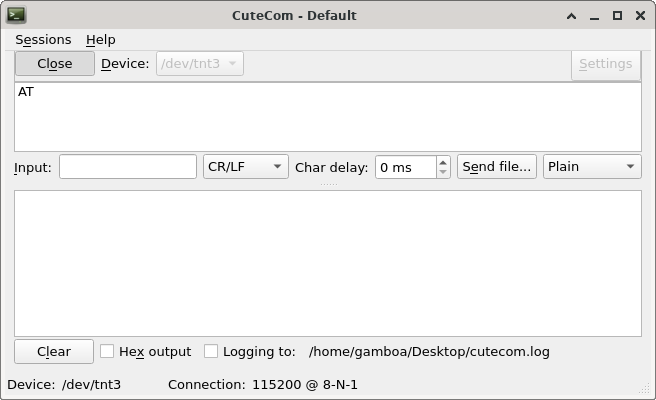
\includegraphics[width=0.8\textwidth]{img/cutecom.png} 
\end{figure} 

A serial terminal is used to send and receive data over a serial communication channel. 
The use of this terminal can be replaced by others like the Arduino IDE serial monitor. 

To use this tool with PICSimLab you first need to configure a virtual serial port as described in Chapter: \hyperlink{def:seriali}{Serial Communication}.
It is possible to use this tool with a real serial port connected to a real device. 


\section {Serial Remote Tank} \hypertarget{def:srtank}{}


The serial remote tank is a tank simulator controlled by a serial communication protocol.
The tank has several sensors and actuators that can be read and controlled using the communication protocol. 
The parameters of the serial communication port must be  19200 8N1. 

\begin{figure}[H]
\center
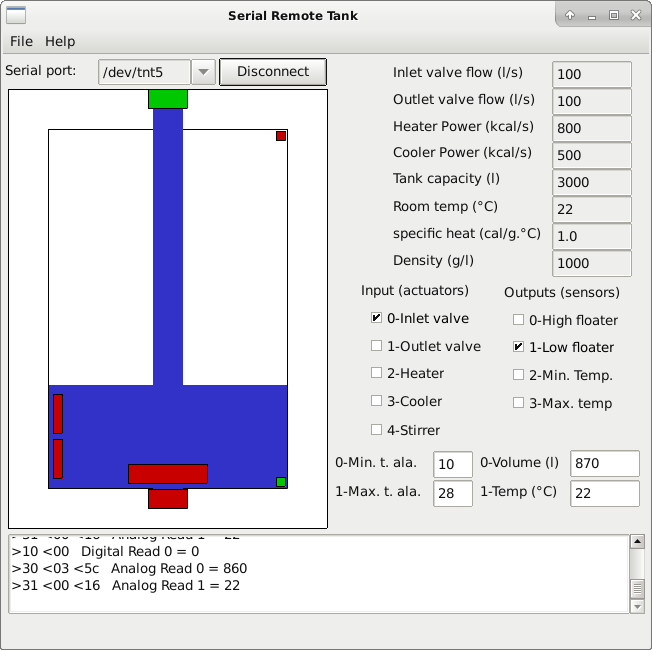
\includegraphics[width=0.8\textwidth]{img/srtank.png} 
\end{figure} 


To use this tool with PICSimLab you first need to configure a virtual serial port as described in Chapter: \hyperlink{def:seriali}{Serial Communication}.
It is possible to use this tool with a real serial port connected to a real device. 

\subsection{Actuators}

Digital inputs:
\begin{enumerate}
\item Inlet valve
\item Outlet valve
\item Heater
\item Cooler
\item Stirrer
\end{enumerate}

Analog inputs:
\begin{enumerate}
\item Minimal temperature alarm trigger level
\item Maximal temperature alarm trigger level
\end{enumerate}

\subsection{Sensors}

Digital outputs:
\begin{enumerate}
\item High floater 
\item Low floater
\item Minimal temperature 
\item Maximal temperature
\end{enumerate}

Analog outputs:
\begin{enumerate}
\item Volume
\item Temperature
\end{enumerate}


\subsection{Communication Protocol}

\subsubsection{Writing on Digital Input}
Sent one byte in 0x0N hexadecimal format where N  is the number of input followed by a second byte with value 0x00 for disable or 0x01 for enable.  

Example to turn on the input 2:
\begin{minted}[baselinestretch=1.2,fontsize=\footnotesize,bgcolor=colorbash]{c}
            Serial_write(0x02);
            Serial_write(0x01);
\end{minted}


\subsubsection{Reading Digital Output}
Sent one byte in 0x1N hexadecimal format where N  is the number of output and read one byte. The byte readed have value 0x00 for disable or 0x01 for enable. 

Example to read output 3:
\begin{minted}[baselinestretch=1.2,fontsize=\footnotesize,bgcolor=colorbash]{c}
      Serial_write(0x13);
      valor=Serial_read(0);
\end{minted}


\subsubsection{Writing on Analog Input} 
Sent one byte in 0x2N hexadecimal format where N  is the number of input followed by two bytes with the 16 bits value.

Example to write the value 230 on analog input 1:
\begin{minted}[baselinestretch=1.2,fontsize=\footnotesize,bgcolor=colorbash]{c}
            Serial_write(0x21);
            valor=230;
            Serial_write((valor&0xFF00)>>8);
            Serial_write(valor&0x00FF);
\end{minted}

\subsubsection{Reading Analog Output}
Sent one byte in 0x3N hexadecimal format where N  is the number of output and read two bytes to form the 16 bits value.

Example to read analog output 2:
\begin{minted}[baselinestretch=1.2,fontsize=\footnotesize,bgcolor=colorbash]{c}
      Serial_write(0x32);
      valorh=Serial_read(0);
      valorl=Serial_read(0);
      valor=(valorh<<8)|valorl;
\end{minted}



\section{Esp8266 Modem Simulator} \hypertarget{def:espmsim}{}


The ESP8266 modem simulator emulates the operation of an esp8266
with wifi modem firmware. Communication is done using a serial channel via 
AT modem commands. 
The parameters of the serial communication port must be  115200 8N1. 

\begin{figure}[H]
\center
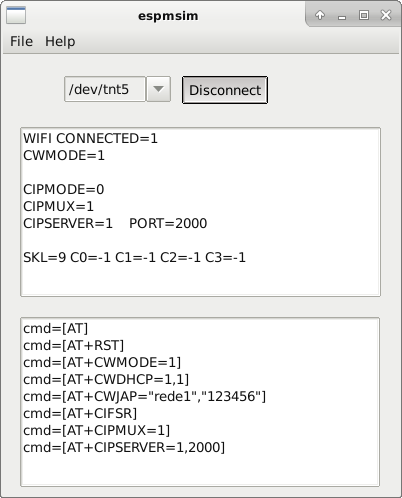
\includegraphics[width=0.7\textwidth]{img/espmsim.png} 
\end{figure} 

To use this tool with PICSimLab you first need to configure a virtual serial port as described in Chapter: \hyperlink{def:seriali}{Serial Communication}.
It is possible to use this tool with a real serial port connected to a real device. 


\subsection{Supported Commands}

\begin{itemize}
\item AT
\item AT+RST
\item AT+GMR
\item AT+CWMODE=1
\item AT+CWDHCP=1,1
\item AT+CWLAP
\item AT+CWJAP="rede1","123456"
\item AT+CIFSR
\item AT+CIPMUX=1
\item AT+CIPSERVER=1,2000
\item AT+CIPSEND=0,10
\item AT+CIPCLOSE=0
\end{itemize}


\section{Arduino Bootloader}\hypertarget{def:aboot}{}

This menu option load PICSimLab microcontroller with Arduino serial bootloader.  
The microcontroller with the bootloader loaded can be programmed directly by the 
Arduino IDE or using the avrdude program. 

To use this tool with PICSimLab you first need to configure a virtual serial port as described in Chapter: \hyperlink{def:seriali}{Serial Communication}.


\section{MPLABX Debugger Plugin} \hypertarget{def:mpdebug}{}

This menu option open the web page to download the MPLABX Debugger Plugin.

The plugin must be installed on MPLABX to allow debugging and programming 
PICSimLab (PICs and AVRs) from the IDE, like a real tool for debugging and 
programming.

\section{Pin Viewer} \hypertarget{def:pinv}{}

 The  PinViewer connects to PICSimLab through the \hyperlink{def:rcontrol}{rcontrol interface} 
 and allows viewing the status and direction of all microcontroller pins. 
 It is also possible to change the state of the digital pins and adjust the
 voltage value on the analog pins configured as input. Pins configured as outputs 
 also show the average value, useful for evaluating the functioning of PWM outputs. 
 
\begin{figure}[H]
\center
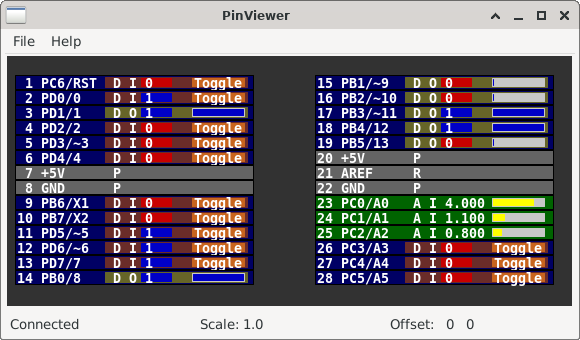
\includegraphics[width=0.7\textwidth]{img/pinviewer.png} 
\end{figure} 

\chapter{Oscilloscope}
 
 The PICSimLab has a basic two-channel oscilloscope that can be used to view the signal on any pin of the microcontroller. The oscilloscope can be accessed through the ``Modules->Oscilloscope'' menu.
 \begin{figure}[H]
\center
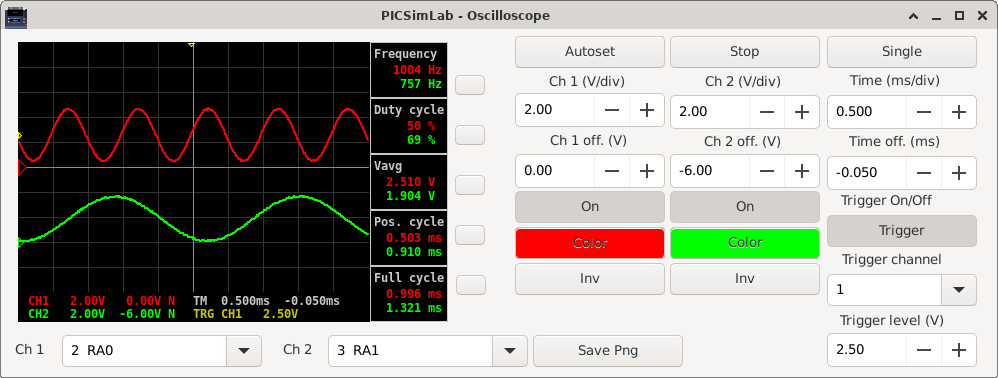
\includegraphics[width=0.99\textwidth]{img/osc.png} 
\end{figure} 




\chapter{Spare Parts} \hypertarget{def:spare}{}

The PICSimLab has a window that allows the connection of spare parts to the microcontroller, it can be accessed through the menu `` Modules-> Spare parts ''.

The main window has the menu with the following functions:
\begin{itemize}
 \item File
 \begin{itemize}
 \item New configuration - Clear the spare parts window 
 \item Save configuration - Saves the current settings of the spare parts into .pcf file
 \item Load configuration - Loads the settings from .pcf file
 \item Save pin alias - Saves the current pin alias to .ppa text file
 \item Load pin alias - Loads the pin alias from .ppa file
\end{itemize}
 \item Edit
 \begin{itemize}
 \item Clear pin alias - Clear the pin alias 
 \item Toggle pin alias - Enable/Disable pin alias use
 \item Edit pin alias - Open current pin alias .ppa file in text editor
 \item Reload pin alias - Reload the current .ppa pin alias file (need after edit .ppa file) 
 \item Zoom in - Increase draw scale
 \item Zoom out - Decrease draw scale
\end{itemize}
 \item Inputs
 \begin{itemize}
  \item Encoder - Adds a rotary quadrature encoder with push button
  \item FM50 (Temperature) - Adds a analog temperature sensor
  \item Fixed Voltage -  Adds a analog fixed voltage reference
  \item Gamepad - Adds a gamepad
  \item Gamepad (Analogic) - Adds a gamepad with one analogic output 
  \item Keypad -  Adds one matrix keypad
  \item LM35 (Temperature) - Adds a analog temperature sensor
  \item MPU6050 - Adds a accelerometer and gyroscope (only raw values)
  \item Potentiometers - Adds 4 potentiometers
  \item Potentiometers (Rotary) - Adds 4 rotary potentiometers
  \item Push Buttons - Adds 8 push buttons
  \item Push Buttons (Analogic) - Adds 8 push buttons with analog output
  \item SHT3X - Adds a analog temperature and humidity sensor
  \item Switchs - Adds eight switchs
  \item Ultrasonic HC-SR04 - Adds a ultrasonic range sensor
\end{itemize}
 \item{Outputs}
  \begin{itemize}
   \item 7 Segments Display -  Adds four multiplexed 7 segments displays
   \item 7 Segments Display (w/dec) -  Adds four multiplexed 7 segments displays with decoder
   \item Buzzer - Adds a active/passive buzzer
   \item DC Motor - Adds a DC motor with H-bridge and quadrature encoder 
   \item LCD hd44780 - Adds a text display hd44780
   \item LCD ili9340 - Adds a color graphic display ili9340 with touchscreen 
   \item LCD pcd8544 - Adds a monochrome graphic display pcd8544 (Nokia 5110)
   \item LCD pcf8833 - Adds a color graphic display pcf8833
   \item LCD ssd1306 - Adds a monochrome graphic display ssd1306
   \item LED Matrix - Adds a 8x8 LED matrix with MAX72xx controller 
   \item LEDs - Adds 8 red LEDs
   \item RGB LED - Adds one RGB LED 
   \item Servo Motor - Adds a servo motor
   \item Step Motor - Adds a step motor
 \end{itemize}
 \item{Others}
  \begin{itemize}
   \item ETH w5500 - Adds a ethernet shield w5500
   \item IO 74xx595 - Adds a 74xx595 SIPO 8 bit shift register
   \item IO MCP23S17 - Adds a MCP23S17 serial SPI IO expander
   \item IO PCF8574 - Adds a PCF8574 serial I2C IO expander
   \item IO UART - Adds a UART serial port 
   \item Jumper Wires - Adds sixteen jumper wires 
   \item MEM 24CXXX - Adds a 24CXXX serial I2C EEPROM  memory
   \item RTC ds1307 - Adds a ds1307 real time clock 
   \item RTC pfc8563 - Adds a pfc8563 real time clock
   \item SD Card - Adds a SD card shield
   \item Temperature System - Adds a temperature control system
  \end{itemize}
\item{Virtual}
  \begin{itemize}
  \item D. Transfer Function - Adds a discrete transfer function mathematical model
  \item IO Virtual term - Adds a virtual serial terminal 
  \item Signal Generator - Adds a virtual signal generator
  \item VCD Dump - Adds a digital value file dump recorder 
  \item VCD Dump (Analogic) - Adds a analog value file dump recorder  
  \item VCD Play - Adds a digital value file dump player  
  \end{itemize}   
 \item Help
 \begin{itemize}
 \item Contents - Open Help window
 \item About - Show message about author and version
\end{itemize}
\end{itemize}


\begin{figure}[H]
\center
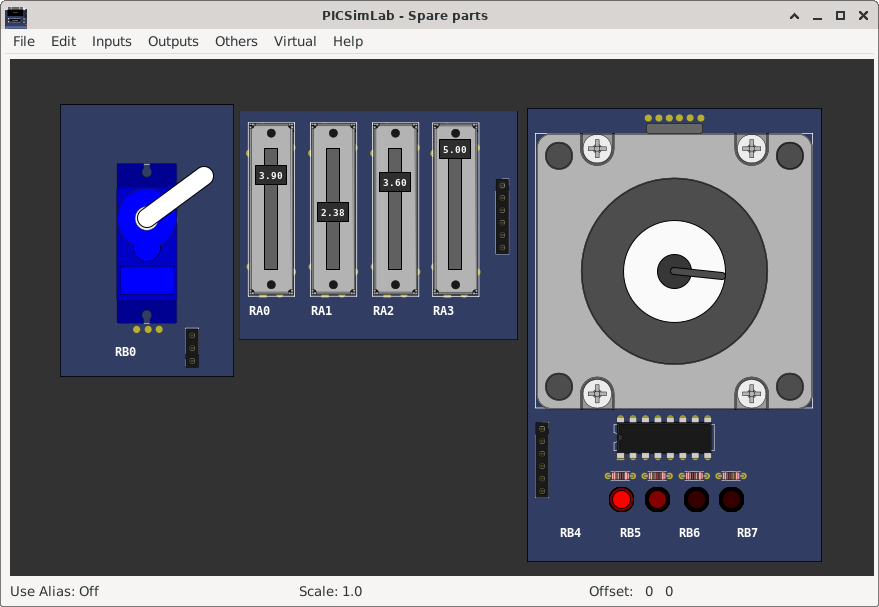
\includegraphics[width=0.99\textwidth]{img/spare.png} 
\end{figure} 

After adding the part, with a right click of the mouse you can access the options menu of the part with the options:
\begin{itemize}
 \item Properties - Opens the connection settings window
 \item Move - Unlocks the part to move
 \item Rotate - Change the orientation of part
 \item Delete - Remove part
 \item Help - Open Help window of part
 \item About - Show message about author and version of part
\end{itemize}


\begin{figure}[H]
\center
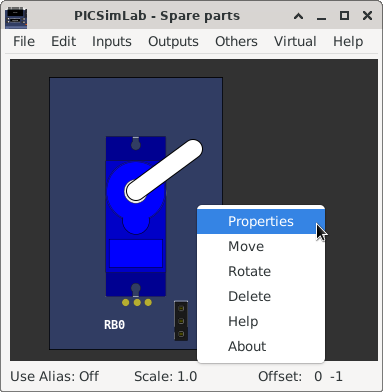
\includegraphics[width=0.60\textwidth]{img/spare_pmenu.png} 
\end{figure} 

\section{Pin Alias}

The pin alias support allows the user to place custom names on the pins making it easy to 
identify according to the project. 

When off the normal names are shown:
\begin{figure}[H]
\center
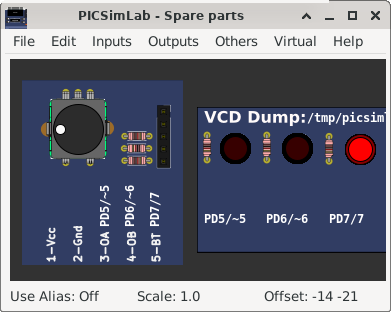
\includegraphics[width=0.80\textwidth]{img/pin_alias_off.png} 
\end{figure} 

When on the alias names are shown:
\begin{figure}[H]
\center
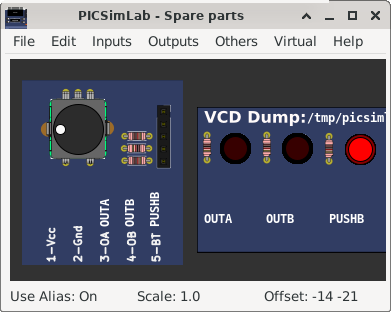
\includegraphics[width=0.80\textwidth]{img/pin_alias_on.png} 
\end{figure} 

To use:
\begin{enumerate}
 \item active the menu ``Edit->Clear pin alias'' to reset the pin alias file
 \item active the menu ``Edit->Edit pin alias'' to open pin alias file, change the names, save and close.
 \item active the menu ``Edit->Reload pin alias'' to load new alias
 \item active the menu ``Edit->Toggle pin alias'' to show new alias
\end{enumerate}


\section{Inputs}
\subsection{Encoder}

This part is a rotary quadrature encoder with push button. The output is twenty pulses per revolution.

\begin{figure}[H]
\center
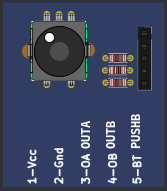
\includegraphics[width=0.25\textwidth]{img/part_encoder.png} 
\end{figure} 

\href{https://lcgamboa.github.io/picsimlab_examples/examples/examples_index.html\#Encoder}{Examples}
 
\subsection{FM50 (Temperature)}

This part is FM50 analog temperature sensor. The measurement range is -40 to 125 °C  and 
voltage output is 10mV/°C + 500mV.

\begin{figure}[H]
\center
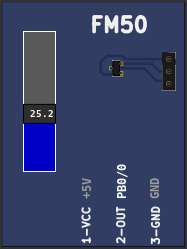
\includegraphics[width=0.3\textwidth]{img/part_fm50.png} 
\end{figure} 


\href{https://lcgamboa.github.io/picsimlab_examples/examples/examples_index.html\#FM50_(Temperature)}{Examples}

\subsection{Fixed Voltage}

This part is analog fixed voltage reference. The value range is 0 to 5V.

\begin{figure}[H]
\center
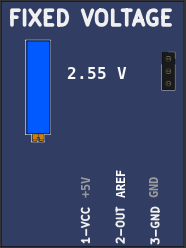
\includegraphics[width=0.3\textwidth]{img/part_fixedv.png} 
\end{figure} 


\href{https://lcgamboa.github.io/picsimlab_examples/examples/examples_index.html\#Fixed_Voltage}{Examples}

 
\subsection{Gamepad}

This part is a gamepad with two analog axis and 7 push buttons.

\begin{figure}[H]
\center
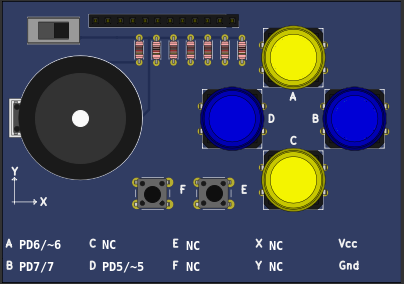
\includegraphics[width=0.6\textwidth]{img/part_gamepad.png} 
\end{figure} 

\begin{figure}[H]
\center
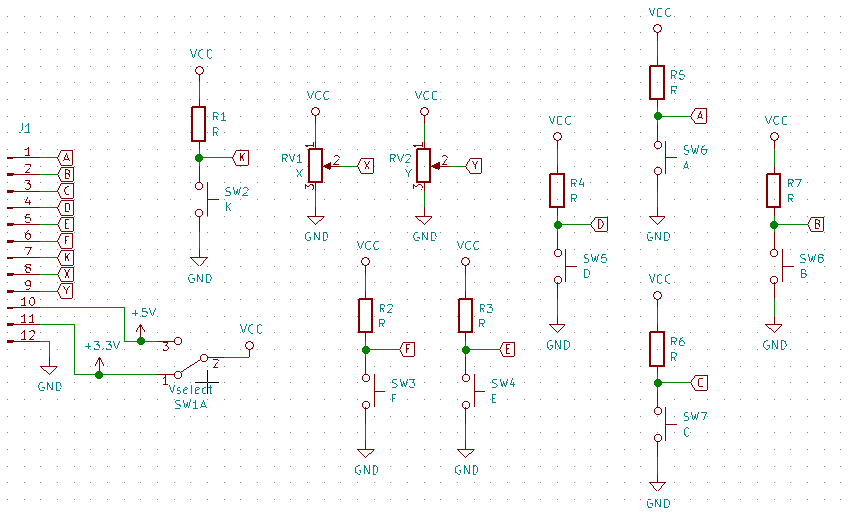
\includegraphics[width=0.99\textwidth]{img/part_gamepad_.png} 
\end{figure} 

The gamepad can be controlled by keyboards keys:
\begin{itemize}
 \item X axis - keys 'A' and 'D'
 \item Y axis - keys 'W' and 'S'
 \item Button A - key 'I'
 \item Button B - key 'L'
 \item Button C - key 'K'
 \item Button D - key 'J'
 \item Button E - key 'E'
 \item Button F - key 'O'
 \item Button K - key 'R'
\end{itemize}


\href{https://lcgamboa.github.io/picsimlab_examples/examples/examples_index.html\#Gamepad}{Examples}

\subsection{Gamepad Analogic}

This part is a gamepad with 5 push buttons and one analogic output.

\begin{figure}[H]
\center
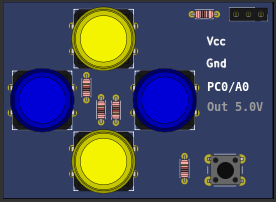
\includegraphics[width=0.4\textwidth]{img/part_gamepad_an.png} 
\end{figure} 


The gamepad can be controlled by keyboards keys:
\begin{itemize}
 \item Button A - key 'L'
 \item Button B - key 'I'
 \item Button C - key 'K'
 \item Button D - key 'J'
 \item Button E - key 'O'
 \end{itemize}


\href{https://lcgamboa.github.io/picsimlab_examples/examples/examples_index.html\#Gamepad_Analogic}{Examples}

\subsection{Keypad}

It is a matrix keyboard configurable to 4x3 , 4x4 or 2x5 rows/columns.

\begin{figure}[H]
\center
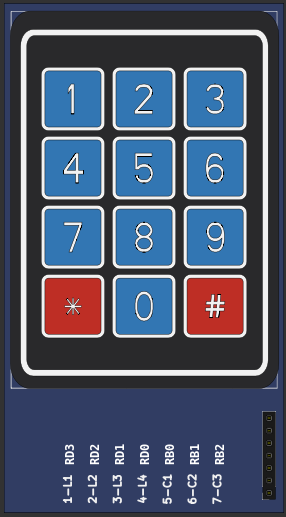
\includegraphics[width=0.33\textwidth]{img/part_keyb_4x3.png} 
\end{figure} 

\begin{figure}[H]
\center
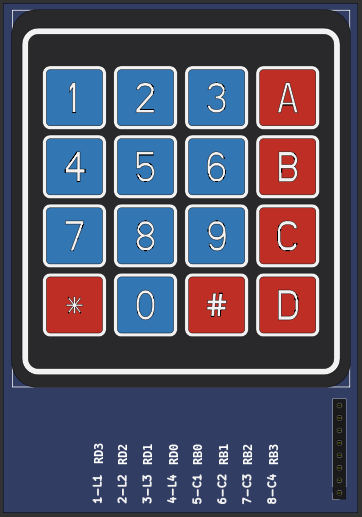
\includegraphics[width=0.4\textwidth]{img/part_keyb_4x4.png} 
\end{figure} 

\begin{figure}[H]
\center
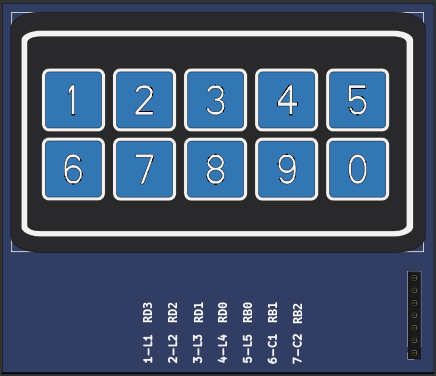
\includegraphics[width=0.5\textwidth]{img/part_keyb_2x5.png} 
\end{figure} 

\href{https://lcgamboa.github.io/picsimlab_examples/examples/examples_index.html\#Keypad}{Examples}

\subsection{LM35 (Temperature)}

This part is LM35 analog temperature sensor. The measurement range is 2 to 150 °C  and 
voltage output is 10mV/°C.

\begin{figure}[H]
\center
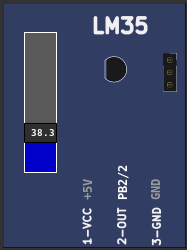
\includegraphics[width=0.3\textwidth]{img/part_lm35.png} 
\end{figure} 


\href{https://lcgamboa.github.io/picsimlab_examples/examples/examples_index.html\#LM35_(Temperature)}{Examples}


\subsection{MPU6050}

This part is MPU6050 accelerometer and gyroscope with I2C interface. 
Only raw values are available, DMP is not supported.

\begin{figure}[H]
\center
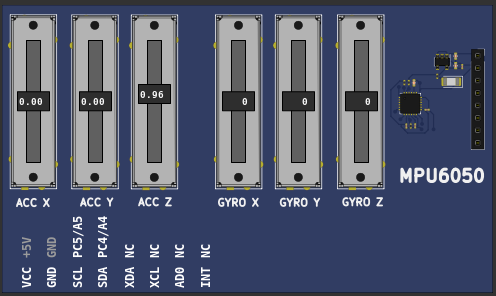
\includegraphics[width=0.6\textwidth]{img/part_mpu6050.png} 
\end{figure} 


\href{https://lcgamboa.github.io/picsimlab_examples/examples/examples_index.html\#MPU6050}{Examples}

\subsection{Potentiometers}

This part is formed by 4 potentiometers connected between 0 and 5 volts, the output is connected to the cursor and varies within this voltage range.
\begin{figure}[H]
\center
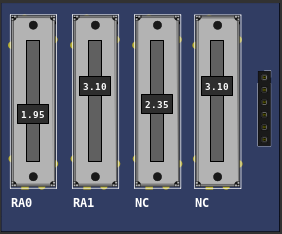
\includegraphics[width=0.6\textwidth]{img/part_pot.png} 
\end{figure} 

\begin{figure}[H]
\center
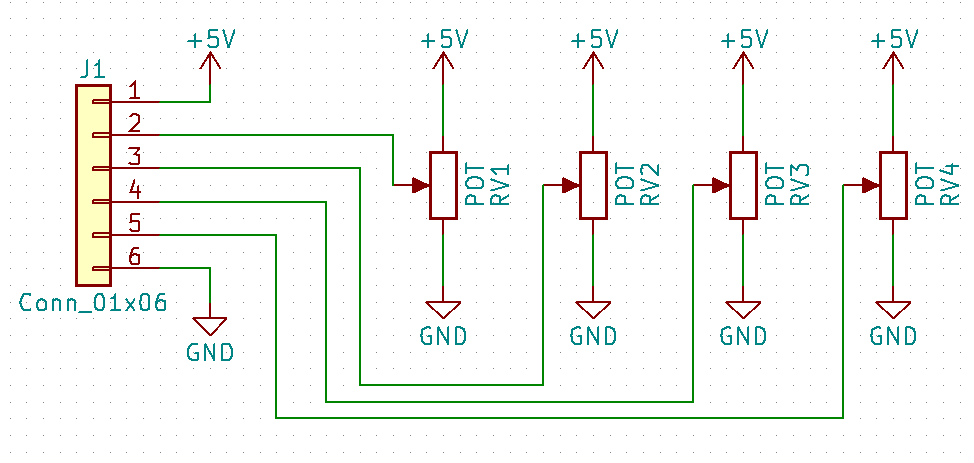
\includegraphics[width=0.8\textwidth]{img/part_pot_.png} 
\end{figure} 

\href{https://lcgamboa.github.io/picsimlab_examples/examples/examples_index.html\#Potentiometers}{Examples}

\subsection{Potentiometers (Rotary)}

This part is formed by 4 rotary potentiometers connected between 0 and 5 volts, the output is connected to the cursor and varies within this voltage range.
\begin{figure}[H]
\center
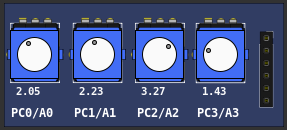
\includegraphics[width=0.6\textwidth]{img/part_pot_r.png} 
\end{figure} 

\begin{figure}[H]
\center
\includegraphics[width=0.8\textwidth]{img/part_pot_.png} 
\end{figure} 

\href{https://lcgamboa.github.io/picsimlab_examples/examples/examples_index.html\#Potentiometers\_(Rotary)}{Examples}

\subsection{Push Buttons}

This part consists of 8 push buttons. The output active state can be configurable.
\begin{figure}[H]
\center
\includegraphics[width=0.99\textwidth]{img/part_buttons.png} 
\end{figure} 

\begin{figure}[H]
\center
\includegraphics[width=0.99\textwidth]{img/part_buttons_.png} 
\end{figure} 

\href{https://lcgamboa.github.io/picsimlab_examples/examples/examples_index.html\#Push\_buttons}{Examples}


\subsection{Push Buttons (Analogic)}


This part consists of 8 push buttons connected in a resistive ladder.

\begin{figure}[H]
\center
\includegraphics[width=0.99\textwidth]{img/part_push_a.png} 
\end{figure}

\href{https://lcgamboa.github.io/picsimlab_examples/examples/examples_index.html\#Push_buttons\_(Analogic)}{Examples}

\subsection{SHT3X (Temp. Hum.)}

This part is SHT3X analog temperature and humidity sensor. The temperature  range is -40 to 125 °C  and 
voltage output is 22.85mV/°C + 1.53V . The relative humidity range is 0 to 100 \%  and voltage output is 40mV/\% + 500mV.

\begin{figure}[H]
\center
\includegraphics[width=0.5\textwidth]{img/part_sht3x.png} 
\end{figure} 


\href{https://lcgamboa.github.io/picsimlab_examples/examples/examples_index.html\#SHT3X_(Temp._Hum.)}{Examples}



\subsection{Switchs}
This part consists of 8 keys with on or off position (0 or 1).

\begin{figure}[H]
\center
\includegraphics[width=0.99\textwidth]{img/part_switchs.png} 
\end{figure} 

\begin{figure}[H]
\center
\includegraphics[width=0.99\textwidth]{img/part_switchs_.png} 
\end{figure} 

\href{https://lcgamboa.github.io/picsimlab_examples/examples/examples_index.html\#Switchs}{Examples}



\subsection{Ultrasonic HC-SR04}
This part is ultrasonic range meter sensor.

\begin{figure}[H]
\center
\includegraphics[width=0.4\textwidth]{img/part_hcsr04.png} 
\end{figure} 


\href{https://lcgamboa.github.io/picsimlab_examples/examples/examples_index.html\#Ultrasonic_HC-SR04}{Examples}



\section{Outputs}

\subsection{7 Segments Display}

This is a four multiplexed 7 segments displays.

\begin{figure}[H]
\center
\includegraphics[width=0.5\textwidth]{img/part_7seg.png} 
\end{figure} 

\href{https://lcgamboa.github.io/picsimlab_examples/examples/examples_index.html\#7\_Segments\_Display}{Examples}

\subsection{7 Segments Display (Decoder)}

This is a four multiplexed 7 segments displays with BCD to 7 segments decoder (CD4511).

\begin{figure}[H]
\center
\includegraphics[width=0.6\textwidth]{img/part_7seg_dec.png} 
\end{figure} 

\begin{figure}[H]
\center
\includegraphics[width=0.5\textwidth]{img/part_7seg_latch.png} 
\end{figure} 

\href{https://lcgamboa.github.io/picsimlab_examples/examples/examples_index.html\#7\_Segments\_Display\_(w/dec)}{Examples}

\subsection{Buzzer}

This is a active/passive buzzer.

\begin{figure}[H]
\center
\includegraphics[width=0.2\textwidth]{img/part_buzzer.png} 
\end{figure} 

\href{https://lcgamboa.github.io/picsimlab_examples/examples/examples_index.html\#Buzzer}{Examples}


\subsection{DC Motor}

This part is DC motor with H-bridge driver and quadrature encoder. 

\begin{figure}[H]
\center
\includegraphics[width=0.3\textwidth]{img/part_dcmotor.png} 
\end{figure} 

\href{https://lcgamboa.github.io/picsimlab_examples/examples/examples_index.html\#DC\_Motor}{Examples}


\subsection{LCD hd44780}

This part is a text display with 2 (or 4) lines by 16 (or 20) columns.

\begin{figure}[H]
\center
\includegraphics[width=0.6\textwidth]{img/part_hd44780_2x16.png} 
\end{figure} 

\begin{figure}[H]
\center
\includegraphics[width=0.7\textwidth]{img/part_hd44780_2x20.png} 
\end{figure} 

\begin{figure}[H]
\center
\includegraphics[width=0.6\textwidth]{img/part_hd44780_4x16.png} 
\end{figure} 

\begin{figure}[H]
\center
\includegraphics[width=0.7\textwidth]{img/part_hd44780_4x20.png} 
\end{figure} 

\href{https://lcgamboa.github.io/picsimlab_examples/examples/examples_index.html\#LCD\_hd44780}{Examples}

\subsection{LCD ili9341}

This part is a color graphic display with 240x320 pixels with touchscreen (xpt2046 controller).
Only 4 SPI mode and 8 bits parallel mode is avaliable.

\begin{figure}[H]
\center
\includegraphics[width=0.7\textwidth]{img/part_lcd_ili9341.png} 
\end{figure} 

\href{https://lcgamboa.github.io/picsimlab_examples/examples/examples_index.html\#LCD\_ili9341}{Examples}


\subsection{LCD pcf8833}

This part is a color graphic display with 132x132 pixels.

\begin{figure}[H]
\center
\includegraphics[width=0.4\textwidth]{img/part_pcf8833.png} 
\end{figure} 

\href{https://lcgamboa.github.io/picsimlab_examples/examples/examples_index.html\#LCD\_pcf8833}{Examples}


\subsection{LCD pcd8544 }

This part is a monochrome graphic display with 48x84 pixels. (Nokia 5110)

\begin{figure}[H]
\center
\includegraphics[width=0.35\textwidth]{img/part_pcd8544.png} 
\end{figure} 

\href{https://lcgamboa.github.io/picsimlab_examples/examples/examples_index.html\#LCD\_pcd8544}{Examples}

\subsection{LCD ssd1306 }

This part is a monochrome oled graphic display with 128x64 pixels. 
The part suport I2C and 4 SPI serial mode.

\begin{figure}[H]
\center
\includegraphics[width=0.35\textwidth]{img/part_lcd_ssd1306.png} 
\end{figure} 

\href{https://lcgamboa.github.io/picsimlab_examples/examples/examples_index.html\#LCD\_ssd1306}{Examples}


\subsection{LED Matrix}

It is a 8x8 LED matrix with MAX72xx controller.

\begin{figure}[H]
\center
\includegraphics[width=0.4\textwidth]{img/part_LED_matrix.png} 
\end{figure}

\href{https://lcgamboa.github.io/picsimlab_examples/examples/examples_index.html\#LED\_Matrix}{Examples}

\subsection{LEDs}

This part is a bar of 8 independent red LEDs.

\begin{figure}[H]
\center
\includegraphics[width=0.99\textwidth]{img/part_leds.png} 
\end{figure} 

\begin{figure}[H]
\center
\includegraphics[width=0.8\textwidth]{img/part_leds_.png} 
\end{figure} 

\href{https://lcgamboa.github.io/picsimlab_examples/examples/examples_index.html\#LEDs}{Examples}
 
\subsection{RGB LED}

This part consists of a 4-pin RGB LED. Each color can be triggered independently.
Using PWM it is possible to generate several colors by combining the 3 primary colors. 
\begin{figure}[H]
\center
\includegraphics[width=0.4\textwidth]{img/part_rgb.png} 
\end{figure} 

\begin{figure}[H]
\center
\includegraphics[width=0.6\textwidth]{img/part_rgb_.png} 
\end{figure} 

\href{https://lcgamboa.github.io/picsimlab_examples/examples/examples_index.html\#RGB_LED}{Examples}

\subsection{Servo Motor}

The servo motor is a component that must be activated with a pulse of variable width from 1ms to 2ms every 20 ms.
A pulse of 1ms positions the servo at -90º, one from 1.5ms to 0º and one from 2ms to 90º.

\begin{figure}[H]
\center
\includegraphics[width=0.4\textwidth]{img/part_servo.png} 
\end{figure} 

\begin{figure}[H]
\center
\includegraphics[width=0.8\textwidth]{img/part_servo_.png} 
\end{figure} 

\href{https://lcgamboa.github.io/picsimlab_examples/examples/examples_index.html\#Servo\_motor}{Examples}


\subsection{Step Motor}

The stepper motor is a component with 4 coils that must be driven in the correct order to rotate the rotor.
Each step of the motor is 1.8º.

\begin{figure}[H]
\center
\includegraphics[width=0.5\textwidth]{img/part_step.png} 
\end{figure} 

\begin{figure}[H]
\center
\includegraphics[width=0.99\textwidth]{img/part_step_.png} 
\end{figure} 

\href{https://lcgamboa.github.io/picsimlab_examples/examples/examples_index.html\#Step\_motor}{Examples}



\section{Others}


\subsection{ETH w5500}

This part is a ethernet shield w5500 with support to 8 sockets simultaneously.

Only TCP/UDP unicast address sockets is supported. 
DHCP is emulated and return a fake ipv4 address.

All listening ports below 2000 are increased by 2000 to avoid operational system services ports. 
For example listening on port 80 becomes 2080. 

w5500 Status Legend:
\begin{center}
\begin{tabular}{l|l|l}
\hline \textbf{1º Letter - Type} & \textbf{2º Letter - Status} & \textbf{3º Letter - Error}\\
\hline
\hline C - Closed & C - Closed & B - Bind\\
\hline T - TCP & I - Initialized & S - Send\\
\hline U - UDP & L - Listen & R - Receive\\
\hline M - MACRAW (don't supported) & S - Syn sent & L - Listen\\
\hline   & E - Established & U - Reuse\\
\hline   & W - Close wait & C - Connecting\\
\hline   & U - UDP & D - Shutdown\\
\hline   & M - MACRAW (don't supported) &   \\
\hline
\end{tabular}
\end{center}

Click on connector to toggle link status.

\begin{figure}[H]
\center
\includegraphics[width=0.6\textwidth]{img/part_w5500.png} 
\end{figure} 

\href{https://lcgamboa.github.io/picsimlab_examples/examples/examples_index.html\#ETH\_w5500}{Examples}
 

\subsection{IO 74xx595}

This is one 74xx595 serial input and parallel output 8 bit shift register.

\begin{figure}[H]
\center
\includegraphics[width=0.6\textwidth]{img/part_74xx595.png} 
\end{figure} 

\href{https://lcgamboa.github.io/picsimlab_examples/examples/examples_index.html\#IO\_74xx595}{Examples}

\subsection{IO MCP23S17}

It is a MCP23S17 serial SPI IO expander part.

\begin{figure}[H]
\center
\includegraphics[width=0.6\textwidth]{img/part_MCP23S17.png} 
\end{figure} 

\href{https://lcgamboa.github.io/picsimlab_examples/examples/examples_index.html\#IO\_MCP23S17}{Examples}

\subsection{IO PCF8574}

It is a PCF8574 serial I2C IO expander.

\begin{figure}[H]
\center
\includegraphics[width=0.6\textwidth]{img/part_pcf8574.png} 
\end{figure} 

\href{https://lcgamboa.github.io/picsimlab_examples/examples/examples_index.html\#IO\_PCF8574}{Examples}


\subsection{IO UART}

This part is a UART serial port. This part connects the hardware/software UART IO pins of microcontroller to
one real/virtual PC serial port. To use virtual port is need to install a virtual port software, as described in \ref{seriali}. 

\begin{figure}[H]
\center
\includegraphics[width=0.6\textwidth]{img/part_uart.png} 
\end{figure} 

\href{https://lcgamboa.github.io/picsimlab_examples/examples/examples_index.html\#IO\_UART}{Examples}


\subsection{Jumper Wires}

This part are formed by sixteen jumper wires. Each jumper has one input and one output.  The jumper input must be connected to one pin output, 
the jumper output can be connected to multiple pin inputs. The jumper can be used to connect microcontroller pins or make connection between 
spare parts pins.   

\begin{figure}[H]
\center
\includegraphics[width=0.6\textwidth]{img/part_jumper.png} 
\end{figure} 

\href{https://lcgamboa.github.io/picsimlab_examples/examples/examples_index.html\#Jumper\_Wires}{Examples}

\subsection{MEM 24CXXX}

It is a 24CXXX serial I2C EEPROM part. There are support to the models 24C04 and 24C512.

\begin{figure}[H]
\center
\includegraphics[width=0.4\textwidth]{img/part_mem24xx.png} 
\end{figure}

\href{https://lcgamboa.github.io/picsimlab_examples/examples/examples_index.html\#MEM\_24CXXX}{Examples}

\subsection{RTC ds1307}

This part is a ds1307 real time clock with serial I2C interface.

\begin{figure}[H]
\center
\includegraphics[width=0.4\textwidth]{img/part_ds1307.png} 
\end{figure}

\href{https://lcgamboa.github.io/picsimlab_examples/examples/examples_index.html\#RTC\_ds1307}{Examples}


\subsection{RTC pfc8563}

This part is a pfc8563 real time clock with serial I2C interface.

\begin{figure}[H]
\center
\includegraphics[width=0.4\textwidth]{img/part_pcf8563.png} 
\end{figure}

\href{https://lcgamboa.github.io/picsimlab_examples/examples/examples_index.html\#RTC\_pfc8563}{Examples}


\subsection{SD Card}

This part is a SD Card shield. It's necessary set one sd card file image before use it. (Click on SD card connector to open file dialog)

On Linux one empty image can be created with this command: 
\begin{verbatim}
 dd if=/dev/zero of=sd.img bs=1M count=32
\end{verbatim}
This empty image can be used with raw sd card access, to work with FAT file system  the image need to be formatted before the use. (using \href{https://github.com/greiman/SdFat/blob/master/examples/SdFormatter/SdFormatter.ino}{SdFormatter.ino} for example) 

\begin{figure}[H]
\center
\includegraphics[width=0.6\textwidth]{img/part_sdcard.png} 
\end{figure} 


\href{https://lcgamboa.github.io/picsimlab_examples/examples/examples_index.html\#SD\_Card}{Examples}


\subsection{Temperature System}

This part is a temperature control system. 
The temperature control system consists of a heating resistor, an LM35 temperature sensor, 
a cooler and an infrared tachometer.


\begin{figure}[H]
\center
\includegraphics[width=0.65\textwidth]{img/part_tempsys.png} 
\end{figure}

\href{https://lcgamboa.github.io/picsimlab_examples/examples/examples_index.html\#Temperature\_System}{Examples}

\section{Virtual}

\subsection{D. Transfer Function}

This is a discrete transfer function mathematical model. 

\begin{figure}[H]
\center
\includegraphics[width=0.9\textwidth]{img/part_dtransferf.png} 
\end{figure} 

\href{https://lcgamboa.github.io/picsimlab_examples/examples/examples_index.html\#D.\_Transfer\_function}{Examples}

\subsection{IO Virtual Term}

This part is a virtual serial terminal. This part can be used to read and write RX/TX pins UART signals.
This part don't need the use or install of virtual serial ports on computer.  
Clik on terminal picture to open the terminal window.

\begin{figure}[H]
\center
\includegraphics[width=0.99\textwidth]{img/part_vterm.png} 
\end{figure} 

\href{https://lcgamboa.github.io/picsimlab_examples/examples/examples_index.html\#IO\_Virtual\_term}{Examples}

\subsection{Signal Generator}

This part is a virtual signal generator with support for sine, square and triangular waves 
generation with amplitude and frequency adjustment.

\begin{figure}[H]
\center
\includegraphics[width=0.4\textwidth]{img/part_sgen.png} 
\end{figure}

\href{https://lcgamboa.github.io/picsimlab_examples/examples/examples_index.html\#Signal\_Generator}{Examples}

\subsection{VCD Dump}

This part is a digital value file dump recorder. The file can be visualized with gtkwave. 

\begin{figure}[H]
\center
\includegraphics[width=0.8\textwidth]{img/part_vcd_dump.png} 
\end{figure}



\begin{figure}[H]
\center
\includegraphics[width=0.99\textwidth]{img/part_vcd_dump_gtkwave.png} 
\end{figure}

\href{https://lcgamboa.github.io/picsimlab_examples/examples/examples_index.html\#VCD_Dump}{Examples}


\subsection{VCD Dump (Analogic)}


This part is a analog value file dump recorder. The file can be visualized with gtkwave.  

\begin{figure}[H]
\center
\includegraphics[width=0.8\textwidth]{img/part_vcd_dump_an.png} 
\end{figure}



\begin{figure}[H]
\center
\includegraphics[width=0.99\textwidth]{img/part_vcd_dump_gtkwave_an.png} 
\end{figure}

\href{https://lcgamboa.github.io/picsimlab_examples/examples/examples_index.html\#VCD_Dump_(Analogic)}{Examples}

 


\subsection{VCD Play}


This part play a VCD file saved from VCD Dump part.  

\begin{figure}[H]
\center
\includegraphics[width=0.8\textwidth]{img/part_vcd_play.png} 
\end{figure}


\href{https://lcgamboa.github.io/picsimlab_examples/examples/examples_index.html\#VCD_Play}{Examples}



\chapter{Troubleshooting}

The simulation in PICSimLab consists of 3 parts:

\begin{itemize}
 \item The microcontroller program
 \item Microcontroller simulation (made by \href{https://github.com/lcgamboa/picsim}{picsim} and \href{https://github.com/buserror/simavr}{simavr})
 \item Simulation of boards and parts
\end{itemize}


When a problem occurs it is important to detect where it is occurring.

One of the most common problems is the error in the microcontroller program. 
Before creating an issue, test your code on a real circuit (even partially) to make sure the problem 
is not there.

Errors in the microcontroller simulation can be detected using code debugging. Any instruction 
execution or peripheral behavior outside the expected should be reported in the project of simulator
used (\href{https://github.com/lcgamboa/picsim}{picsim} or \href{https://github.com/buserror/simavr}{simavr}).

If the problem is not in either of the previous two options, the problem is probably in PICSimLab.
A good practice is to send a source code together with a PICSimLab workspace (.pzw file) to open the
issue about the problem.




\chapter{License}

Copyright © 2021 Luis Claudio Gambôa Lopes <lcgamboa@yahoo.com>

This program is free software; you can redistribute it and/or modify
it under the terms of the GNU General Public License as published by
the Free Software Foundation; either version 2 of the License, or
(at your option) any later version.

This program is distributed in the hope that it will be useful,
but WITHOUT ANY WARRANTY; without even the implied warranty of
MERCHANTABILITY or FITNESS FOR A PARTICULAR PURPOSE. See the
GNU General Public License for more details.

You should have received a copy of the GNU General Public License
along with this program; if not, write to the Free Software
Foundation, Inc., 59 Temple Place, Suite 330,
Boston, MA 02111-1307, USA.

\appendix
\chapter{Online Simulator}

The online version of PICSimLab has the same source code as the desktop version compiled using 
\href{https://emscripten.org/}{Emscripten}. The online version does not have the Tools menu, support for 
debugging and serial communication (only for \hyperlink{def:vterm}{IO Vterm}). 

\begin{figure}[H]
\center
\includegraphics[width=0.99\textwidth]{img/online.png} 
\end{figure} 

There are three versions generated with Emscripten: 

\begin{itemize}
\item \href{https://lcgamboa.github.io/js/picsimlab_mt.html}{WASM with multithread} - Fast speed (50\% of desktop version )
and worse browser compatibility (currently only tested and work in Chrome and Firefox desktop)
\item \href{https://lcgamboa.github.io/js/picsimlab_wasm.html}{WASM} - Good speed and good browser compatibility
\item \href{https://lcgamboa.github.io/js/picsimlab_asmjs.html}{ASM.JS} - Slow speed and better browser compatibility
\end{itemize}

Clicking on the three-bar menu (botton left) or any loading option in the menus to open the 
file loading window.
Files can be loaded by drag and drop or by the load button. 

\begin{figure}[H]
\center
\includegraphics[width=0.99\textwidth]{img/online2.png} 
\end{figure} 

The simulator can also be accessed from the \href{https://lcgamboa.github.io/picsimlab_examples/examples_index.html}{examples page} for online viewing of most examples (View Online link). 

Due to the limitations of the online version, it is advisable to use the desktop version which has more resources and higher simulation speed, especially above 8Mhz clocks. 

\chapter{Use with MPLABX}

Use with MPLABX to program and Debug

\section{Installing the Necessary Tools}

\subsection{Install MPLABX IDE and XC8 Compiler}
Links for download  \href{http://www.microchip.com/mplabx}{MPLABX IDE} and \href{http://www.microchip.com/compilers}{XC8 Compiler} installers.
Download and install.

\subsection{Install PICsimLab}

Link for download \href{http://sourceforge.net/projects/picsim/files/picsim/picsim-0.6/}{PICsimLab-0.6} installer. 
Download and install

\subsection{How to Install PicsimLab MPLABX Debugger plugin}

Link for download \href{http://sourceforge.net/projects/picsim/files/picsim/picsim-0.6/}{PicsimLab MPLABX Debugger plugin (com-picsim-picsimlab.nbm)} 

\begin{figure}[H]
\center
\includegraphics[width=0.98\textwidth]{img/hmd/mplab01.png} 
\end{figure} 

\begin{figure}[H]
\center
\includegraphics[width=0.8\textwidth]{img/hmd/mplab02.png} 
\end{figure} 

\begin{figure}[H]
\center
\includegraphics[width=0.98\textwidth]{img/hmd/mplab03.png} 
\end{figure} 

\begin{figure}[H]
\center
\includegraphics[width=0.6\textwidth]{img/hmd/mplab04.png} 
\end{figure} 

\begin{figure}[H]
\center
\includegraphics[width=0.98\textwidth]{img/hmd/mplab05.png} 
\end{figure} 


\begin{figure}[H]
\center
\includegraphics[width=0.7\textwidth]{img/hmd/mplab06.png} 
\end{figure} 

\begin{figure}[H]
\center
\includegraphics[width=0.7\textwidth]{img/hmd/mplab07.png} 
\end{figure} 

\begin{figure}[H]
\center
\includegraphics[width=0.7\textwidth]{img/hmd/mplab08.png} 
\end{figure} 

\begin{figure}[H]
\center
\includegraphics[width=0.7\textwidth]{img/hmd/mplab09.png} 
\end{figure} 


\section{Configuring a New Project in MPLABX}

\subsection{Project Creation}

\begin{figure}[H]
\center
\includegraphics[width=0.98\textwidth]{img/hmd/mplab10.png} 
\end{figure} 

\begin{figure}[H]
\center
\includegraphics[width=0.71\textwidth]{img/hmd/mplab11.png} 
\end{figure} 

\begin{figure}[H]
\center
\includegraphics[width=0.71\textwidth]{img/hmd/mplab12.png} 
\end{figure}

\begin{figure}[H]
\center
\includegraphics[width=0.71\textwidth]{img/hmd/mplab13.png} 
\end{figure} 

\begin{figure}[H]
\center
\includegraphics[width=0.71\textwidth]{img/hmd/mplab14.png} 
\end{figure} 

\begin{figure}[H]
\center
\includegraphics[width=0.71\textwidth]{img/hmd/mplab15.png} 
\end{figure} 

\begin{figure}[H]
\center
\includegraphics[width=0.71\textwidth]{img/hmd/mplab16.png} 
\end{figure} 

\subsection{File Creation}

\begin{figure}[H]
\center
\includegraphics[width=0.98\textwidth]{img/hmd/mplab17.png} 
\end{figure} 

\begin{figure}[H]
\center
\includegraphics[width=0.8\textwidth]{img/hmd/mplab18.png} 
\end{figure} 


\subsection{PIC Configuration Bits}
\begin{figure}[H]
\center
\includegraphics[width=0.98\textwidth]{img/hmd/mplab19.png} 
\end{figure} 

\begin{figure}[H]
\center
\includegraphics[width=0.98\textwidth]{img/hmd/mplab20.png} 
\end{figure} 


\begin{figure}[H]
\center
\includegraphics[width=0.98\textwidth]{img/hmd/mplab21.png} 
\end{figure} 

\subsection{Code Example}

Paste the configuration and this simple code example in test.c:
\begin{minted}{c}
void main()
{
    TRISB=0x00; //All pins as output
    PORTB=0;    //All pins off
    while(1)    //main loop
    {
        PORTBbits.RB0=1; //Turn RB0 on
        PORTBbits.RB1=1; //Turn RB1 on
        PORTB=0;  //All pins off
    }
}
\end{minted}


\begin{figure}[H]
\center
\includegraphics[width=0.98\textwidth]{img/hmd/mplab22.png} 
\end{figure} 

\subsection{Building the Project}

Use the \textbf{Build} button and wait for the message ``\textcolor{green}{BUILD SUCCESSFUL}''.

\begin{figure}[H]
\center
\includegraphics[width=0.98\textwidth]{img/hmd/mplab23.png} 
\end{figure} 



\section{Program and Debug PICsimLab With MPLABX}


\subsection{Starting PICsimLab}
\begin{figure}[H]
\center
\includegraphics[width=0.8\textwidth]{img/hmd/mplab24.png} 
\end{figure} 

The plugin connect to Picsimlab through a TCP socket using port 1234, and you have to allow the access in the firewall. Verify in the PICsimLab statusbar the message ``MplabxD: Ok''. It's show debugger server state.


\subsection{Programming PICsimLab}

Use the \textbf{Debug} button to programming PICsimLab.  
\begin{figure}[H]
\center
\includegraphics[width=0.98\textwidth]{img/hmd/mplab25.png} 
\end{figure} 

\subsection{Pausing the Program}
Use the \textbf{Pause} button to stop the program and inspect the code and memory.
\begin{figure}[H]
\center
\includegraphics[width=0.98\textwidth]{img/hmd/mplab26.png} 
\end{figure} 

\subsection{Restarting the Program}
Use the \textbf{Restart} button to restart the program.
\begin{figure}[H]
\center
\includegraphics[width=0.98\textwidth]{img/hmd/mplab27.png} 
\end{figure} 

\subsection{Running Step by Step}
Use the \textbf{Step} or \textbf{Step Over} button to run the program step by step.
\begin{figure}[H]
\center
\includegraphics[width=0.98\textwidth]{img/hmd/mplab28.png} 
\end{figure} 

See in the PICsimLab the changes of each step.
\begin{figure}[H]
\center
\includegraphics[width=0.8\textwidth]{img/hmd/mplab29.png} 
\end{figure} 

\subsection{Stopping Debugger}
Use the \textbf{Stop} button to turn off the MPLABX debugger. The program continues running in PICsimLab after MPLABX debugger is stopped.
\begin{figure}[H]
\center
\includegraphics[width=0.98\textwidth]{img/hmd/mplab30.png} 
\end{figure} 


\section{This Tutorial in Video}

Link for Youtube video version of this tutorial: \href{https://youtu.be/q2oZB50Avm4}{How to use MPLABX to program and debug PicsimLab 0.6}



\chapter{Creating New Boards}

First get the source code and compile as described in \hyperlink{def:isource}{Install from source}.

\section{Creating a New Board}

The first step is get the schematic and all information about the board hardware.
The second step is the creation of four files in PICSimLab dir (consider replace the 'x' of board\_x for a name of your board in your case):
\begin{itemize}
\item Board Picture (share/boards/X/board.svg) or (share/boards/X/board.png);
\item Board map (share/boards/X/board.map);
\item Board header (src/boards/board\_x.h);
\item Board C++ code (src/boards/board\_x.cc);
\end{itemize}

The third and last step is recompiling PICSimLab with new board support.

\subsection{Board Hardware and Schematic}

For this tutorial, the board created have the hardware shown in diagram below:
\begin{figure}[H]
\center
\includegraphics[width=0.7\textwidth]{img/hb/blocks.eps} 
\end{figure} 

The schematic for the tutorial board made in \href{http://kicad-pcb.org/}{Kicad}.
\begin{figure}[H]
\center
\includegraphics[width=0.99\textwidth]{board_x/board_x.eps} 
\end{figure} 

\pagebreak
And the PCB layout was made in \href{http://kicad-pcb.org/}{Kicad} too. The PCB is not necessary if you have a real board.

\begin{figure}[H]
\center
\includegraphics[width=0.9\textwidth, angle=0]{board_x/board_x_pcb.eps} 
\end{figure} 

\pagebreak
\subsection{Board Picture}

The PNG board picture was taken from \href{http://kicad-pcb.org/}{Kicad} 3D viewer.
The picture image is saved as ``share/board/X/board.png''.

\begin{figure}[H]
\center
\includegraphics[width=0.8\textwidth]{files/share/board.png} 
\end{figure} 

It is also possible to use images in SVG format for better viewing quality. 
\href{https://github.com/yaqwsx/PcbDraw}{PCBDraw} can be used to convert a Kicad PCB project to 
an SVG image. 
The picture image is saved as ``share/board/X/board.svg''.
\begin{figure}[H]
\center
\includegraphics[width=0.8\textwidth]{files/share/board_svg.png} 
\end{figure} 

\pagebreak
\subsection{Picture map}
The PICSimLab use one picture image map for inputs and outputs. 

The inputs are the areas in board picture which user can interact (by mouse click) and 
start with letters ``I\_''. 

The output are the areas in board picture to be redraw according simulator status and start with
letters ``O\_''. 

The bidirectional areas in board picture which user can interact and need to be redraw according simulator status 
are started with letter ``B\_''. 

The picture map used for PICSimLab are normal HTML image-map. They can be made by hand or using any software which 
can handle image maps. The original PICSimLab maps are made using \href{http://www.gimp.org/}{Gimp image editor}.     

To start, in the GIMP, use the Filters->Web->Image Map to open image map editor window.
\begin{figure}[H]
\center
\includegraphics[width=0.99\textwidth]{img/hb/gimp01.png} 
\end{figure} 

\pagebreak
Then select rectangle or circle map on toolbar.
\begin{figure}[H]
\center
\includegraphics[width=0.8\textwidth]{img/hb/gimp02.png} 
\end{figure} 

And mark the area in picture.
\begin{figure}[H]
\center
\includegraphics[width=0.8\textwidth]{img/hb/gimp03.png} 
\end{figure} 

\pagebreak
After area is select, in the settings windows select the link type for ``Other''. 
\begin{figure}[H]
\center
\includegraphics[width=0.7\textwidth]{img/hb/gimp04.png} 
\end{figure} 

And write the name of area. The name must describe the area function on the board 
and follow the \hyperlink{def:map}{Picture Map Reference}.

\begin{figure}[H]
\center
\includegraphics[width=0.7\textwidth]{img/hb/gimp05.png} 
\end{figure} 


\subsubsection{Board map}

For this tutorial board, twelve areas are marked:
\begin{itemize}
\item I\_PG\_ICSP - where user click to load hexfile.
\item I\_SW\_PWR - where user click to turn on/off the board.
\item B\_SW\_D1 - Switch connected in RD1.
\item B\_PO\_1 - Potentiometer connected to RA0.
\item B\_PB\_RST - Button to reset board.
\item B\_PB\_D0 - Button connected in RD0. 
\item O\_LD\_LD0 - draw LED connected in push button D0.
\item O\_LD\_LD1 - draw LED connected in switch D1.
\item O\_LD\_LPWR - draw power LED indicator.
\item O\_LD\_RB1  - draw LED connected in RB1.
\item O\_LD\_RB0  - draw LED connected in RB0.
\item O\_IC\_CPU  - draw microcontroller name.
\end{itemize}


\begin{figure}[H]
\center
\includegraphics[width=0.7\textwidth]{img/hb/gimp06.png} 
\end{figure} 


Board map generated by Gimp image map editor and saved as ``share/boards/X/board.map''.
\inputminted[baselinestretch=1.2,fontsize=\footnotesize,linenos]{html}{files/share/board.map}

The kicad project files can be download from github \href{https://github.com/lcgamboa/picsimlab_docs/tree/main/kicad/board_x}{PICSimLab repository}. 

\subsection{Board code}

The header file and c++ code file with comments are listed in the next two subsections. This files control the behavior of board in simulator.

\subsubsection{board\_x.h}

\href{https://github.com/lcgamboa/picsimlab/blob/master/src/boards/board_x.h}{ board\_x.h online file}.

\href{https://lcgamboa.github.io/picsimlab_docs/devel/html/index.html#binc}{ board\_x.h online doxygen version}.


\inputminted[baselinestretch=1.2,fontsize=\footnotesize,linenos,bgcolor=colorbash]{c++}{files/board_x.h}

\pagebreak
\subsubsection{board\_x.cc}

\href{https://github.com/lcgamboa/picsimlab/blob/master/src/boards/board_x.cc}{ board\_x.cc online file}.

\href{https://lcgamboa.github.io/picsimlab_docs/devel/html/index.html#bcode}{ board\_x.cc online doxygen version}.

\inputminted[baselinestretch=1.2,fontsize=\footnotesize,linenos,bgcolor=colorbash]{c++}{files/board_x.cc}


\subsection{Integration with PICsimLab}


After include the four files created for new board, the PICSimLab can be recompiled,
as described in \hyperlink{def:isource}{Install from source}.


\subsection{Final Result}

The PICSimLab board created for this tutorial are shown in the figure below.
\begin{figure}[H]
\center
\includegraphics[width=0.9\textwidth]{img/hb/final.png} 
\end{figure} 

The sample program below can be used to test new board, this code is write for XC8 compiler:
\inputminted[baselinestretch=1.2,fontsize=\footnotesize,linenos]{c}{sample/board_x.c}





\end{document}
